\chapter{Generation, benchmarks and evaluation}\label{ch:GBEM}

\minitoc% Creating an actual minitoc

\par Since styles are ill-defined, they can not be evaluated explicitly (we can not quantify them in advance). Thus, we need a proxy method in order to implicitly evaluate them. We can do this by using them in order to generate behaviors (i.e., synthesis handwriting traces), and evaluate the quality of those behaviors relative to the ground-truth behaviors (i.e., the original letters traces). In other words, to study styles, we would like to reconstruct the target behaviors using generative models, only informed by the task and the styles to perform the behavior. In this chapter, we discuss the recent advances in neural generative models: how are they trained? how do we infer from them? Then we look at paradigm for reconstruct target behaviors, with focus on the usage of neural networks.

\par After we generate the behaviors, we need to evaluate them in a manner that evaluates the styles. This is still an open research question, and a complicated one as well. It also goes hand-in-hand with the choices made in generative models. We discuss the used evaluation metrics across different domains (e.g., text, speech and handwriting evaluation). We also discuss the difficulties associated with finding the suitable evaluation metric.

\par We then present the experiments done in order generate drawings and ground our proposed evaluation metrics. We will explain our choices for the model design, the inference methods, and our approach to ground the metrics.

% \par This chapter sets the foundation for the PhD.

\begin{mdframed}[backgroundcolor=blue!20]
    \begin{center}
        Questions addressed in this chapter
    \end{center}

    \begin{itemize}
        \item How to generate handwritten letters using deep learning framework?
        \item How to evaluate the generated traces?
        \item What benchmarks are suitable to compare to?
    \end{itemize}
\end{mdframed}

\clearpage

\section{Background}\label{sec:gbem_background}
\par We start by introducing the different basis for our work in the literature. Most of this work uses deep learning and generative models. How and why deep learning emerged in the last few years is quite important to keep in mind, since it is the starting point for any successful usage of deep learning. We then explore a particular aspect of deep learning: generative models. In particular, we focus on the domain of sequential data, where the problem gets more challenging. A direct consequence for using generative models is the challenge of evaluating what is generated. Generation, after all, has an artistic aspect, unlike well-defined machines learning tasks like regression and classification. We try to make sense of what exists in the literature, and try to deduce what would be a good criteria for evaluation metrics for a generative task.
% \subsection{Deep Learning: quick overview}
% \textbf{\textsc{this part will be modified. focus only on RNN, leave generative models to the next section}}
% \setlist{nolistsep}\begin{itemize}[noitemsep]
%     \item Talk about deep learning and its current uses in general
%     \item
% \end{itemize}

\par Deep learning is a subset of machine learning~\citep{lecun2015deep,Goodfellow-et-al-2016}, mainly applicable on neural networks. These set of techniques perform remarkably well nowadays on a wide range of tasks and benchmarks (for example, in image recognition~\citep{krizhevsky2012imagenet,simonyan2014very,he2016deep}, speech synthesis~\citep{oord2016wavenet}, image segmentation, handwriting recognition, image captioning~\citep{DBLP:journals/corr/VinyalsTBE14,karpathy2015deep}, language translation~\citep{sutskever2014sequence}, even outperforming humans in some of them (GO game~\citep{silver2016mastering}).

% \GB{I would distinguish between recognition tasks (that discard irrelevant variability) and generation/prediction tasks (that have to deal with output variability)}
% \OSM{07/06: Noted. Will update it.}

% Before deep learning, in order to use machine learning algorithms were good to find patterns, given good features. This task, referred to as \textit{feature engineering}, was quite challenging in many applications (like identifying objects in images for example \textbf{PUT SOME REFERENCES HERE}), and require specific skills related to the domain of interest.

\par Before deep learning, in order to use classical machine learning algorithms, an important step was \textit{feature engineering}: extracting the relevant features from the data, in order to get the relevant information needed to perform the task. In images, techniques like \textit{Scale-invariant feature transform} (SIFT)~\citep{lowe1999object}, and in speech, feature like \textit{Mel-frequency cepstrum} (MFCC) and \textit{Probabilistic  Linear  Discriminate  Analysis} (PLDA)~\citep{narang2015speech}, were quite dominant at that time. There is no one solution that fits all here; it depends on the task in hand, and that required experience. Thus, feature engineering was quite challenging.

The advantage of deep learning techniques is that it overcome (to a big extent) the need for the daunting task of feature engineering. Instead, it tries to learn, from the raw data, hierarchy of features, that are optimal in order to solve the task in hand (i.e., it performs \textit{automated feature engineering}). In our work for example, we did not need to do any kind of temporal feature extraction\footnote{When it comes to spatial features, we performed feature-extraction using Freeman codes and Speed modalities, as discussed in the previous chapter.}.

\par A detailed discussion into the basics of deep learning is out of the scope of this document (and has been done properly in many books and tutorial available online). We refer you to the book~\citep{Goodfellow-et-al-2016} for more theoretical treatment of deep learning, and to~\citep{chollet2017book,geron2017hands} for a more practical aspect.
% GB: not fan:
%\textbf{Write about the history of deep learning, and how did it become the way it is now - algorithmic\citep{srivastava2014dropout}, hardware, data, software frameworks and language... -}

\subsection{Sequential data} \label{sec:seq_data}
\par Sequential data appears in a lot of our daily life, for example: text, speech, the weather status, etc. In a more formal manner, a sequential data example is formed of tokens, and can be represented as $x_1, x_2, ..., x_N$, where $x_n$ is one token, and $N$ is the total length of this sequential data point.

\par Let's take a more concrete example: text. We have multiple sentences in a given text. We can consider each sentence as a data point/example. If we consider an example sentence: \textit{the cat is eating the food}, and we define our tokens to be the words\footnote{There is no rule here for how we define the tokens. We can, for example, define the letters to be our tokens. In the case of text, it is a trade-off: considering words as tokens allow the model to be more fluent, but it also means that the learning space is very large (sometimes the number of unique words to predict at each time step is in the order of tens of thousands). If we consider letters as tokens however, it makes the model job more tractable (all the letters, symbols, digits, can be in the order of tens), but it leads to less quality for the model.}. In this case, $x_1=the$, $x_2=cat\dots\,etc$.

\par What is common between all the sequential data (and what also distinguish them from non-sequential data points) is that each token is dependent on the previous token/s. In general, when we want to model sequential data, we in essence want to learn the following probability distribution:
\begin{equation}
    p(x_1, x_2, ..., x_N) = p(x_1) \times p(x_2|x_1) \times p(x_3|x_2, x_1) \times .... \times p(x_N|x_1 ... x_{N-1})
    \label{eq:rnn_obj_training_0}
\end{equation}

\par In order to model such a distribution using neural networks, we can either:
\begin{enumerate}
    \item Adding a \textit{state variable} in order to factorize the problem. In this case, we introduce an intermediate state variable, $h$, which model the dependency on the previous tokens. Our objective in this case will be
    \begin{equation}
        p(h_n) = p(h_{n-1}, x_{n})
        \label{eq:rnn_factorization}
    \end{equation}
    This can be done using \textit{Recurrent Neural Networks} (RNN), which will be explained later in detail (section~\ref{sec:RNN}). In this case, the network is looping over the tokens one-by-one, updating the state variable each time.
    \item Use the whole sequential data (all its tokens) as input to the network in the same time. In this case, the network is trying to model equation~\ref{eq:rnn_obj_training_0} heads-on. This approach has gained popularity recently with the work done in~\citep{oord2016wavenet,gehring2017convolutional}, using convolution networks in order to model sequential data (signals for the first and text for the second). The advantages of this approach is removing the sequential aspect of the network, and leveraging parallelism when treating the whole sequence. This results in faster training, while still achieving state-of-the art results.
\end{enumerate}

\par There is no one solution that fits all here, it simply depends on the problem and the constraints on the solution. In case of variable-length sequential data, the first approach is the one to go for. In the case of fixed-length sequential data, the second approach should be considered (easier to train the model, faster to optimize, faster to infer from).

\subsection{Recurrent Neural Networks and Sequence Modeling} \label{sec:RNN}
As mentioned briefly in the previous section (\ref{sec:seq_data}), \textit{Recurrent Neural Networks} (RNN) is a type of neural networks, that can handle sequential aspect in data. In its simplest format, it is a simple feed-forward network, applied on each token in the sequential data point, while carrying the information about the previous tokens using a latent variable $h$, commonly referred to as \textit{the hidden state variable}. This is demonstrated in figure~\ref{fig:basic_rnn_model}.

\begin{figure}
    \centering
    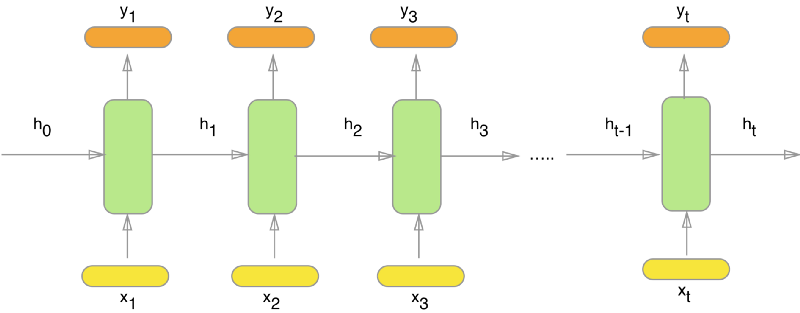
\includegraphics[width=\textwidth]{images/gbem/basic_rnn.png}
    \caption{A demonstration of how RNN works: the network is applied on each token in the input ($x_1, x_2, ..., x_t$), while update the hidden state variable every time ($h_0, h_1, ..., h_t$). The output at each step is a function of the hidden state variable (not demonstrated here). Source of the image is from~\citep{howrnnworks}.}
    \label{fig:basic_rnn_model}
\end{figure}

\par To describe it in a more formal manner, let's first assume the following:
\begin{itemize}
    \item The input $x$ is first processed by a set of weights, $W_{ih}$, and bias $b_{ih}$.
    \item From each step to the other, the hidden state $h$ is processed via a set weights, $W_{hh}$, and bias $b_{hh}$.
    \item Last, the output is given by processing the hidden state $h$ via another set of weights, $W_{ho}$, and bias $b_{ho}$.
\end{itemize}

\par If we assume that output activation is a simple linear layer (thus, it is a regression task), then the equations of this simple RNN are the following:
\begin{align}
    \begin{split}
    z_n = W_{ih} \cdot x_{n} + b_{ih}
    \\
    h_n = W_{hh} \cdot [h_{n-1}, z_{n}] + b_{hh}
    \\
    y_n = W_{ho} \cdot h_{n} + b_{ho}
    \label{eq:rnn_equations}
    \end{split}
\end{align}

\par Where the brackets $[\ ]$ indicate a concatenation process. In case of a simple regression task, a typical loss function is the \textit{Minimum Square Error}, which can be formulated as:
\begin{equation}
    Loss = \frac{1}{T \times N} \sum_{n}^{N} \sum_{t}^{T} \left ( y_{n, t} - \hat{y_{n, t}}\right )^2
    \label{eq:loss_fn_mse}
\end{equation}
where $T$ is the length of the sequence, and the $N$ is the number of sequential data points available, and $\hat{y_{n, t}}$ is predicted output by the model, while $\hat{y_{n, t}}$ is the ground truth output.

\par Given this formalization, the objective is to find the set of weights and biases of the network, that will minimize the chosen loss function. We will explore the optimization algorithms in section~\ref{subsec:optimization}.

\subsection{Optimization Algorithms} \label{subsec:optimization}
% \par One of the important factors in the recent success of deep learning is the advances in optimization algorithms. These algorithmic advances make the optimization easier, converge to a better solution, and require less tweaking in order to achieve a good performance. All these methods are derivatives of stochastic gradient descent optimization~\citep{robbins1951stochastic}., defined as~\citep{gradientdescent}:
\par One of the important factors in the recent success of deep learning is the advances in optimization algorithms. These algorithmic advances make the optimization easier, converge to a better solution, and require less tweaking in order to achieve a good performance. All these methods are derivatives of gradient descent optimization~\citep{boyd2004convex}.
%
% \begin{quote}
%     Gradient descent is a first-order iterative optimization algorithm for finding the minimum of a function. To find a local minimum of a function using gradient descent, one takes steps proportional to the negative of the gradient (or approximate gradient) of the function at the current point.
% \end{quote}

\par If the function to be optimized is convex~\citep{ben2001lectures} -- differentiable, and have a global optima --, then gradient descent can find this global optima. An example for the different optimization iteration can be seen in figure~\ref{fig:grad_descent}.

\begin{figure}
    \centering
    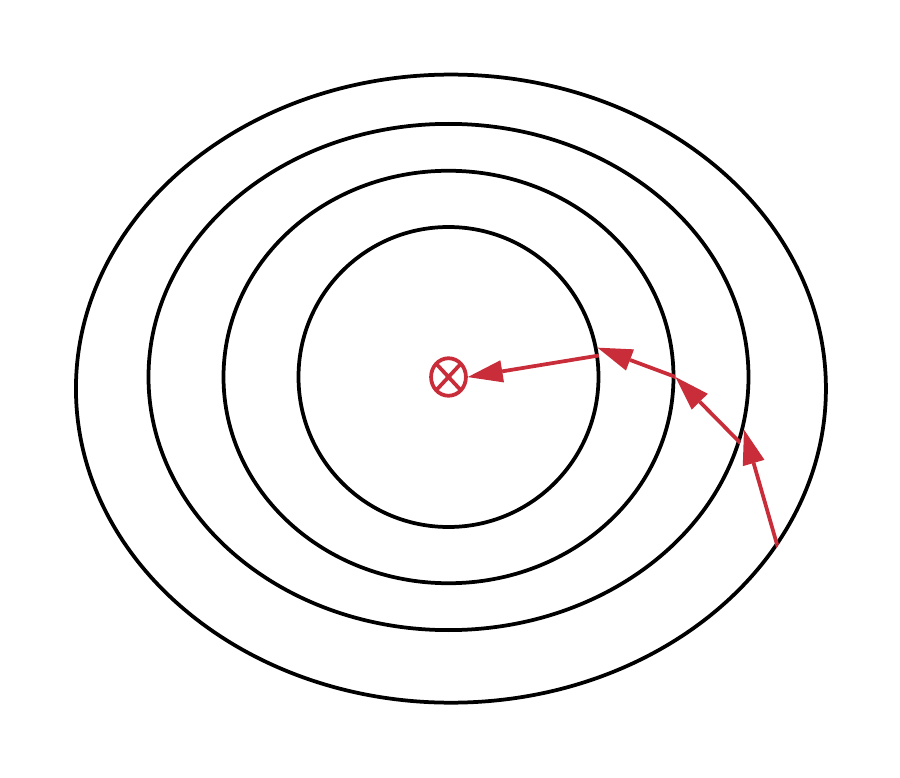
\includegraphics{images/gbem/grad_descent.png}
    \caption{A demonstration for how a gradient descent algorithm work. The optimization process progress each step towards the global optima (the indicated point in the center).}
    \label{fig:grad_descent}
\end{figure}

\par Gradient descent can be formalize by the following equation:
\begin{equation}
    % \theta_{t+1} = \theta_{t} - \alpha \times \dv{Loss(\theta_t)}{\theta_t}
    \theta_{t+1} = \theta_{t} - \alpha \times \frac{d Loss(\theta_t)}{d\theta_t}
    \label{eq:grad_descent}
\end{equation}
where $\theta$ refers to the parameters we want to optimize, $t,t+1$ refers to the current and the next iterations respectively, $\alpha$ is the learning rate (how large the step to take at each iteration), and $Loss$ is the loss/objective function we want to optimize our parameter for. Optimization by gradient descent is a \textit{batch optimization}: the loss function and its gradient is calculated all given data examples. This iterative process keeps going till we do not observe a tangible change in the performance of the parameters, or we exhaust our computational budget. An illustration for this process can be seen in figure~\ref{fig:grad_descent_inuitive}.

\begin{figure}
    \centering
    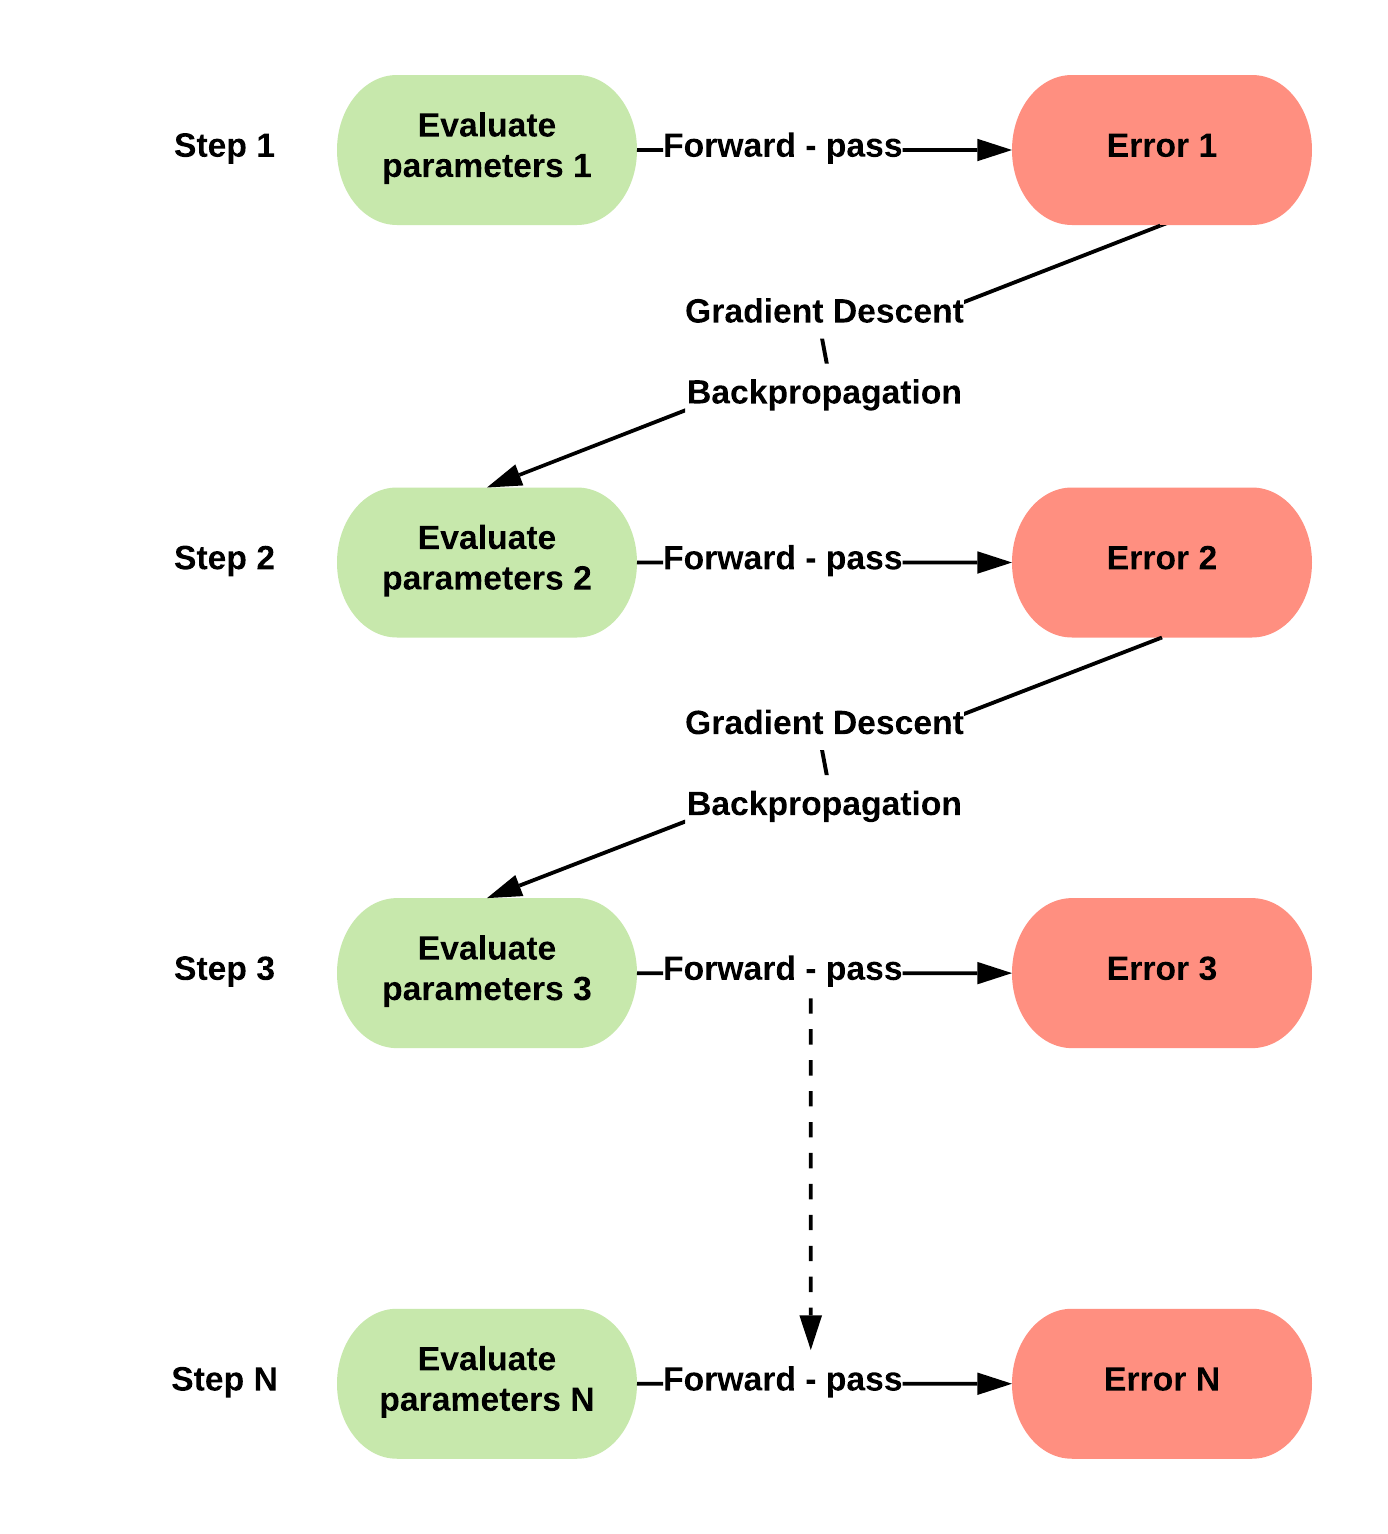
\includegraphics{images/gbem/gradient_descent_informal.png}
    \caption{The process of gradient descent is iterative, and include 3 steps: evaluate the quality of the current parameters (forward-pass step), get the error value, use the error-value in order to update the parameters/getting new set of parameters (\textit{Back-Propagation} step). This process is repeated N times, which is decided by either not observing any update in the error, or we ran out of computational resources.}
    \label{fig:grad_descent_inuitive}
\end{figure}

\par In case of recurrent neural networks, an adaptation from of \textit{Back-Propagation} step is used, called \textit{Back-Propagation Through Time} (BPTT)~\citep{werbos1988generalization,robinson:utility,mozer1995focused}. It simply works by unfolding the recurrent neural network to the length of the input sequence -- with each copy of the network having the same parameters --, and then apply the normal \textit{Back-Propagation} step consequently on each step, in order to find the proper network parameters.

Before we dive into the different optimization methods currently used, it is important first to stress on an important characteristic of all modern deep neural networks, which are~\citep{Goodfellow-et-al-2016}:
\begin{itemize}
    \item \textbf{Differentiability}: All the components of the neural networks (activation function, loss objective, regularization, ...etc) are differentiable components. This issue is not about mandatory by theory, but by convenience: good optimizers exist that can use this feature in order to optimize the network faster, while being able to scale with appropriately with the given number of data points and the number of parameters to be optimized.
    \item \textbf{Non-convexity}: While the neural network is built of convex parts, the composition of those parts together is not convex. The reasoning for this particular point is out of the scope of this document. We refer you to the book~\citep{Goodfellow-et-al-2016} for more details --. While this seems to be a disadvantage, it is actually a powerful advantage of the neural network. Neural networks are \textit{universal approximators}, meaning that they can approximate/learn any function. A convex function can not approximate non-convex function, but the other way around works~\citep{lecture_nn_optimization}.

    Using gradient descent optimization methods in this case leads to convergence to local optima points. The initial conditions of the network (the initial random parameters, and the strategy of their selection) and the optimization strategy and parameters (learning rate, decay factor...,etc) will play an important rule to determine the convergence characteristics (speed of convergence, and local optima) of the neural network.
\end{itemize}

% \subsubsection{Mini-batch optimization}
\par Another important aspect of the success of deep learning is the availability of large amount of data. To optimize the parameters of a deep neural network (can be the order of millions of parameters) using large amount of data (can be in the order of millions of data examples) using gradient descent, is not physically feasible. We do not have the hardware capability to process all of these data in the same time.

\par To get around this issue, \textit{mini-batch} optimization is used: instead of performing gradient descent based on the information from the whole data, we divide the data into chunks (mini-batches). For each mini-batch, we calculate the loss and the gradient, and update the parameters, and then move on the next batch. The gradient descent in this case is called \textit{Stochastic Gradient Descent}, SGD,~\citep{robbins1951stochastic}, following the same equation~\ref{eq:grad_descent}, but applied to only a mini-batch at a time, instead of the whole data (batch).

\par Many advances built on top of SGD helped in advancing deep learning, like combining SGD with momentum~\citep{rumelhart1988learning}, RMSProp algorithm~\citep{hinton2012neural} and Adam algorithm~\citep{kingma2014adam}.

%TODO: Not sure if I should keep and expand this part, or no.
% \subsection{Architectures}
% \OSM{INCOMPLETE PART}
%
% In section~\ref{sec:RNN}, we discussed the idea behind the basic RNN and its operation. Then, in section~\ref{subsec:optimization}, we how we can optimize the parameters of a neural network in general.
%
% \par One important aspect of RNN is the ability to keep the information over many time-steps. This is an issue however with basic RNN networks. This can happen with a better choice of the architecture, that allow to keep the memory, which also learning to select what is not necessary to keep (what we can forget). This problem is called \textit{vanishing gradient}.
%
% A formal discussion for \textit{vanishing gradient} is extensively and better treated in many resources. To get an intuition for it, let's re-phrase what gradient descent optimization is actually doing: the network parameters are evaluated over the data, giving us an error value (the evaluation of the loss function). Using this error value, we move/update the parameters of the network in a direction that minimizes the future error. We keep repeating these steps till we no further improvement is observed (or we exhausted our computational budget). In RNN,
%
% Talk about Vanilla RNN (and what is their problem), LSTMs (and the intuition behind then in solving the problems), and then GRUs (simpler than LSTMs -- fewer parameters --, yet perform similar)

% \subsection{Back-propagation through time}

% \subsection{Training a generator}


\subsection{Inference: How to generate sequences from the network?}
\par There exists several approaches in order to generate information from the networks. In the case of recurrent neural networks, this is a sequential process (one step at a time, till we generate the whole sequence), as illustrated in figure~\ref{fig:text_gen}.

\begin{figure}
    \centering
    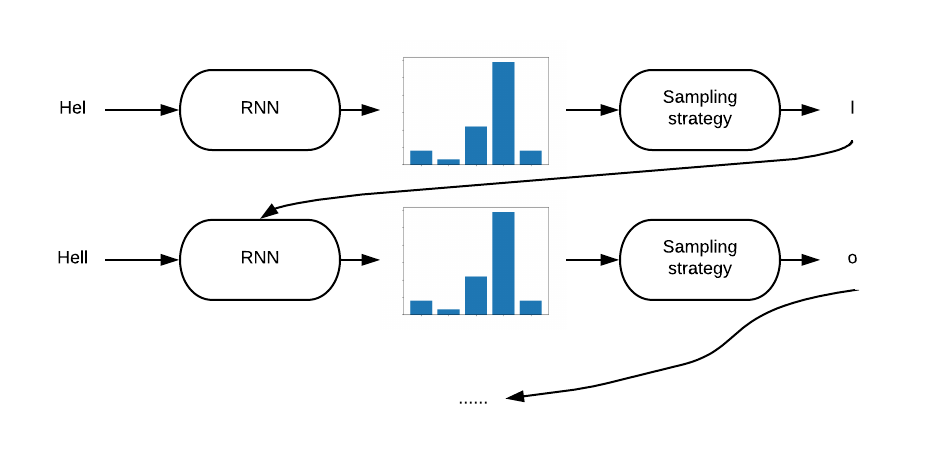
\includegraphics{images/gbem/text_gen.png}
    \caption{An example of using RNN in order to infer a sentence. The token to be generated here is a character. At each time step, the model is given the part of the sentence that has been generated so far, and asked to give the probability distribution over the next character. This distribution is then given to the selected sampling distribution, which sample the next character, and so on.}
    \label{fig:text_gen}
\end{figure}

During the inference mode, the objective is to generate the most likely sequence. We want to solve the following problem

\begin{equation}
    \begin{split}
    \textrm{Find $x_1, x_2, ..., x_N$ that }\\
    {argmax}_{x_1, x_2, ..., x_N}p(x_1, x_2, ..., x_N)
    \label{eq:rnn_obj_inf}
    \end{split}
\end{equation}

% \par Unfortunately, this problem is not tractable, as it scales badly with the number of options (i.e, dimensions) per time step, and the number of time steps required. Multiple methods are being used currently to find an approximate solution to this problem \GB{I would order from the simplest to the most complex}: beam search, temperature sampling, and greedy selection.
% \paragraph{Beam Search} \GB{Describe: selection of N best candidates at each time step of the forward pass given the past and perform a back-pass picking up the best solution}
% \paragraph{Temperature Sampling} \GB{Sample the distribution up to a certain threshold} Since the output of the network is discrete, we use a $SoftMax$ function in order to model this distribution\footnote{The concept of temperature sampling is not limited to the discrete distributions only. You can use it to sample from a \textit{Gaussian Mixture Model} (GMM) for example. In that case, higher temperatures smooth the difference in the weights between the different Gaussian distributions during the sampling process.}.
% \paragraph{Greedy Selection} is a special case of temperature sampling, $T = 0$. In other words, for every time-step, we sample value with the highest probability (e.g., like in the training paradigm). The advantage of this scheme is that it is deterministic and computationally cheap, thus easy to reproduce. The disadvantage on the other side is, like other greedy algorithms, it is sub-optimal, thus yielding worse results.

\par This problem, however, is not tractable, as it scales badly with the number of options (i.e, dimensions) per time step, and the number of time steps required. One simple way is to perform \textit{greedy sampling}, where, at each time step, we select the most likely token. This, however, leads to repetitive and predictable patterns~\citep{chollet2017book}.

\par A better way will be to use \textit{stochastic sampling}, by leveraging the fact that at each step, we have a probability distribution over all possible tokens. This allows more diversity in the generated tokens, and also allow unlikely tokens to be sampled some of the time.

\par But what if we want to control the level of randomness in the sampling process? Having such control will allow us to explore different ways to infer from the model, in order to determine the most satisfying way. This control can be done using \textit{temperature sampling}. The idea is to reshape the probability distribution over the different token. On one extreme, very high temperature (going to infinity) will flatten the distribution, making the distribution equivalent to \textit{uniform distribution}. On the other extreme, a temperature of zero will be mount to greedy sampling. This is illustrated in figure~\ref{fig:temperature_sampling}.

\begin{sidewaysfigure}[!htbp]
    \centering
    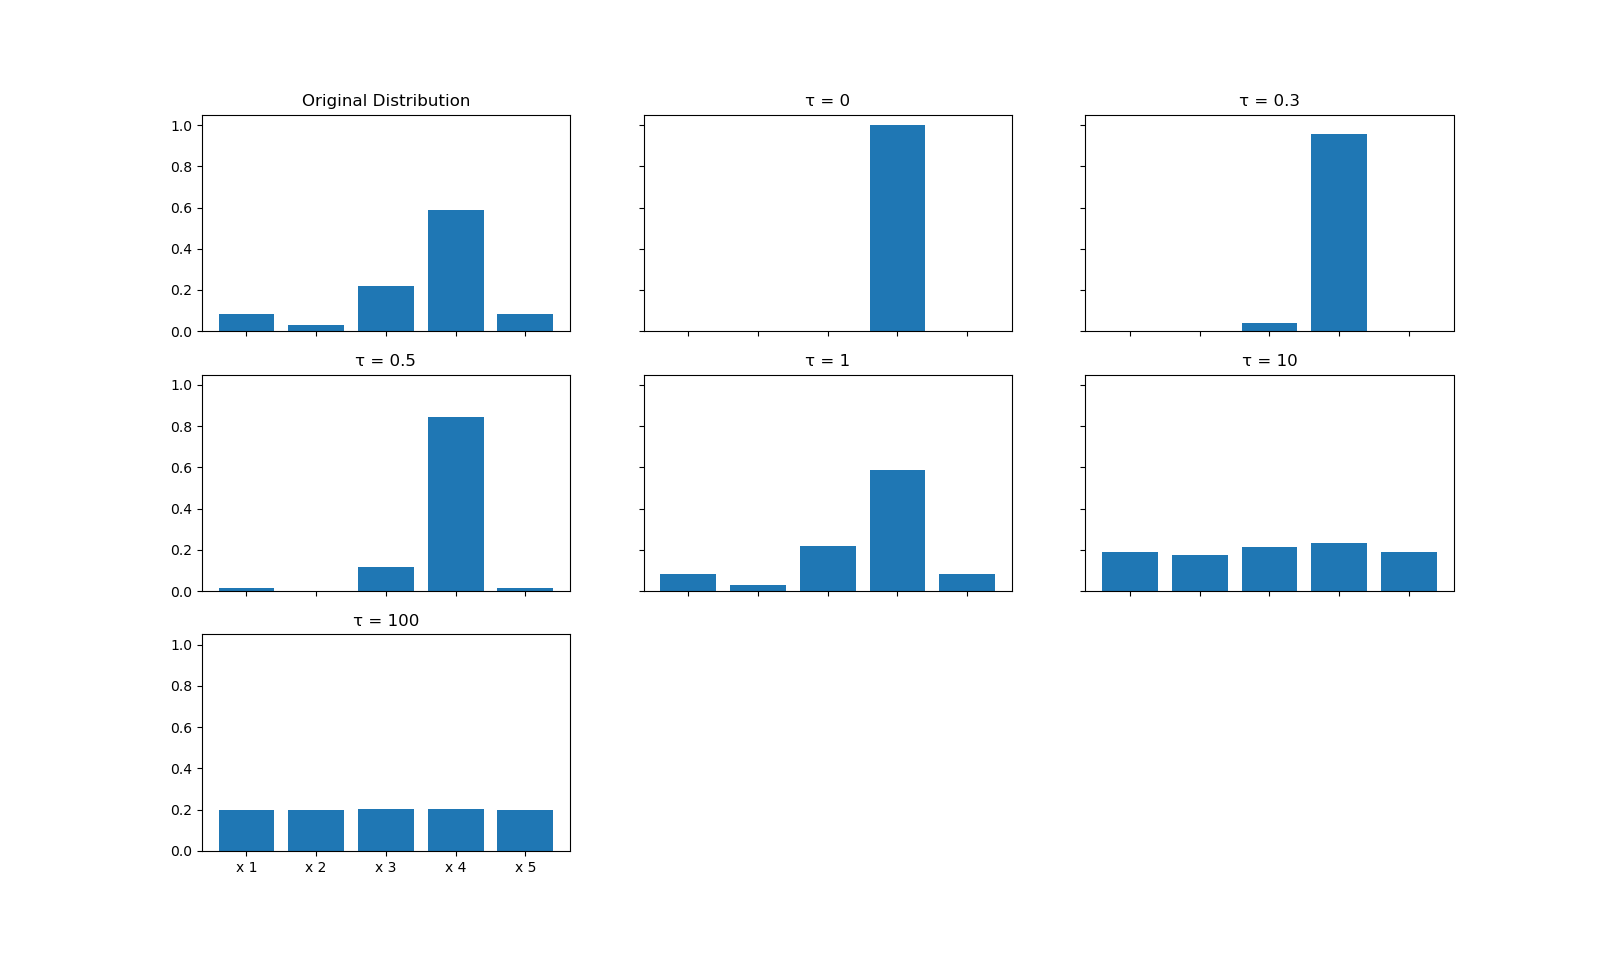
\includegraphics[scale=0.5]{images/gbem/temperature_sampling.png}
    \caption{Illustration of temperature sampling. When the temperature $\tau$ is very low, it becomes greedy sampling. With the increase of temperature, we can see more higher possibility of sampling the lower-probability tokens. When the temperature is too high, it becomes uniform sampling.}
    \label{fig:temperature_sampling}
\end{sidewaysfigure}

\par A clear advantage for temperature sampling is its simplicity, ease of implementation, and ability to generate diverse outputs. However, this also create a challenge when we want to focus on issues like repeatability and reproducibility.

\par Another important thing to notice is that the training/optimization part is not the same as the generation part. Usually in machine learning, there is a symmetry between the training and testing procedures. However, in generation, we are suddenly letting the model generate long sequences, and use it output from the current step as the input to the next step. The model is not trained to see its own output in the input. It is trained to see always the ground truth in the input. Overtime, there is an accumulation of errors that build up, leading to the degradation in the quality of generation~\citep{DBLP:journals/corr/RanzatoCAZ15}. This discrepancy between the training and generation will have consequences in the evaluation process, as we will see shortly.

\subsection{How to introduce prior to the model? (conditioning the model)}
\par When training a RNN network, we usually initialize the first hidden state with zeros. This way, we are informing the model that we are not making any prior assumptions about that particular sequence, and that all sequences in the data have the same 'no prior assumption' condition.

\par However, what if you want to add some prior knowledge about the sequence to the model? There are two reasons why we may want to do that:
\begin{itemize}
    \item Increase accuracy: In case we are doing some classic pattern recognition task (classification, regression), having extra useful information will definitely help increasing the model final performance.
    \item Act as a command: In case of generative model -- during the generative mode -- we need a way to \textit{trigger} the model in order to start generating a sequence in a particular context. For example, we want to tell the model to generate letter 'A'.  Initializing the model with this value allow it to start generating letter A.
\end{itemize}

There are multiple ways to bias the model, all targeting the same thing: initializing the hidden state of the model. Some work in the literature combines multiple of these approaches in the same setup. To the best of our knowledge, there is no one place which all these methods are discussed together.

\paragraph{Initialize the first hidden state directly} This is a common approach, used image captioning~\citep{karpathy2015deep}, machine translation, and sequence-to-sequence autoencoders. This is illustrated in figure~\ref{subfig:hidden_state}.

\paragraph{Using the first time-step} This method was used in the work done in~\citep{vinyals2015show}, in the area of image captioning. The prior in this case is the image, and the objective is to generate the text caption for it. In order to condition the model, the authors projected the image information into the same size as the word embedding used, thus creating a \textit{fake} word, and concatenated this new word with the rest of the words. The hidden state after this fake word is now condition on the information from the image. This is illustrated in figure~\ref{subfig:first_timestep}.

\paragraph{Using context sequence -- multiple time-steps --} In this approach, the model is provided with some time-steps from the ground truth, in give it a context. At the end of the these given time-steps, the hidden state is initialized with information about what to be done. A use case for this scenario -- for example -- is when training a language model on multiple authors. When asking the model to generate, you can provide some sentences from the author you want, so the model can follow on this.

\paragraph{Concatenating input time-steps with the condition} In the work done by~\citep{ha2017neural}, although not mentioned explicitly, the dataset used -- the \textit{QuickDraw} dataset, discussed earlier -- is quite complicated -- they choose different tasks than us --. It is hard to make the model remember the information about such a complex task over a long time span. Thus, the authors use a mix of \textit{initializing the first hidden state} and \textit{concatenating with the first time-step} in order to make it easier for the model to remember the task. This is illustrated in figure~\ref{subfig:cat_timestep}.

\paragraph{Concatenating the hidden state with the condition} This approach is more popular now, since it allows the use of \textit{attention mechanisms}~\citep{NIPS2010_4089,denil2012learning}. Examples for this in image captioning~\citep{xu2015show}, speech synthesis~\citep{wang2017tacotron}.

\begin{figure}
    \centering
    \begin{subfigure}[b]{\textwidth}
      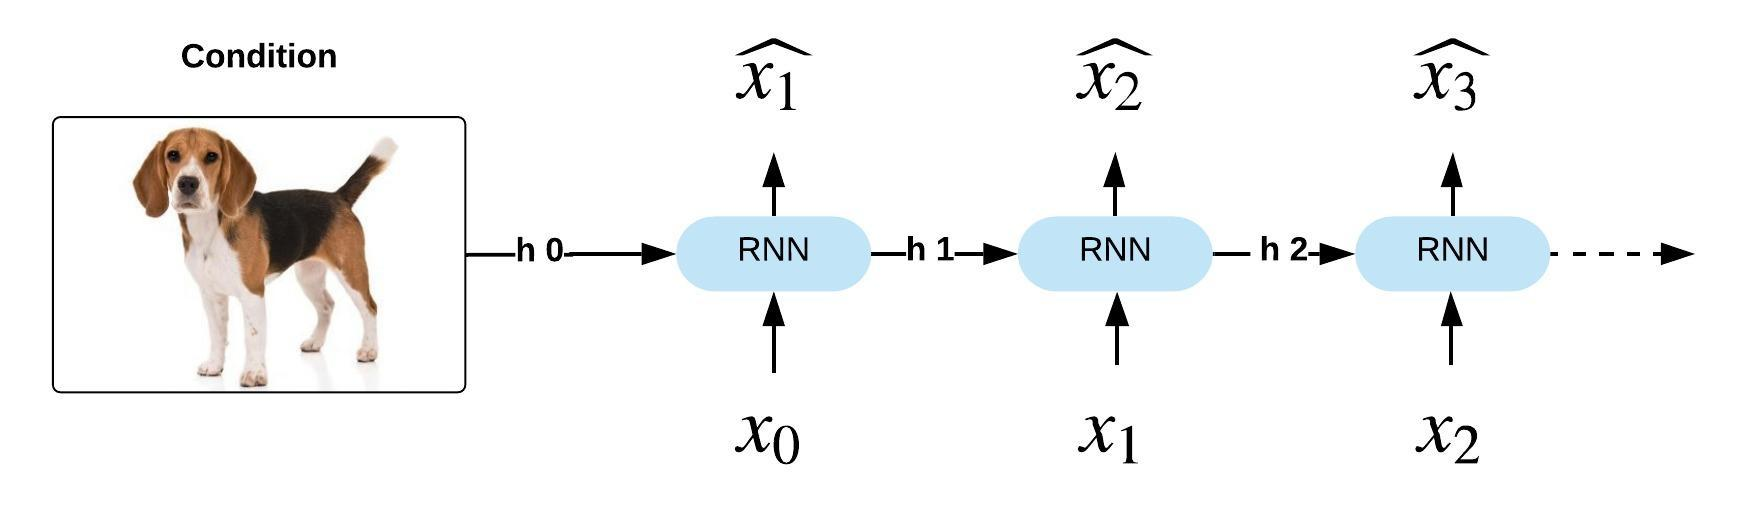
\includegraphics[width=\textwidth]{images/gbem/conditioning_model/hidden_state.jpeg}
      \caption{Initializing the hidden state, similar to the one used in~\citep{karpathy2015deep}.}
      \label{subfig:hidden_state}
    \end{subfigure}
    ~
    \begin{subfigure}[b]{\textwidth}
        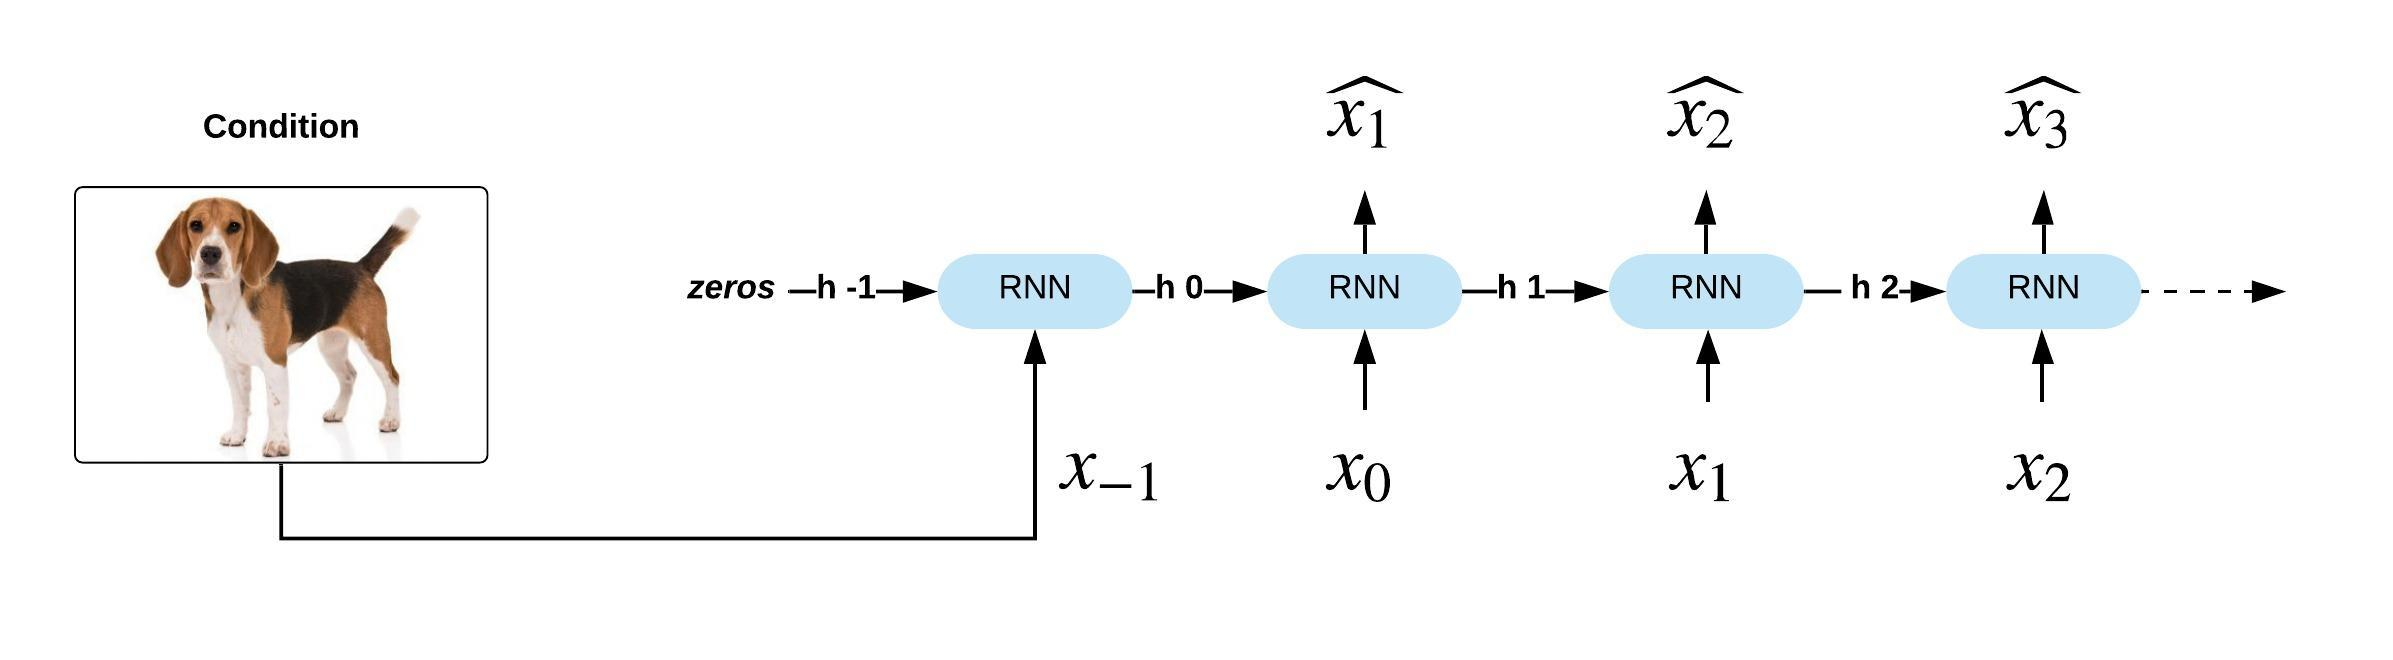
\includegraphics[width=\textwidth]{images/gbem/conditioning_model/first_timestep.jpeg}
        \caption{Initializing using the first time-step, similar to the one used in~\citep{vinyals2015show}.}
        \label{subfig:first_timestep}
    \end{subfigure}
    ~
    \begin{subfigure}[b]{\textwidth}
        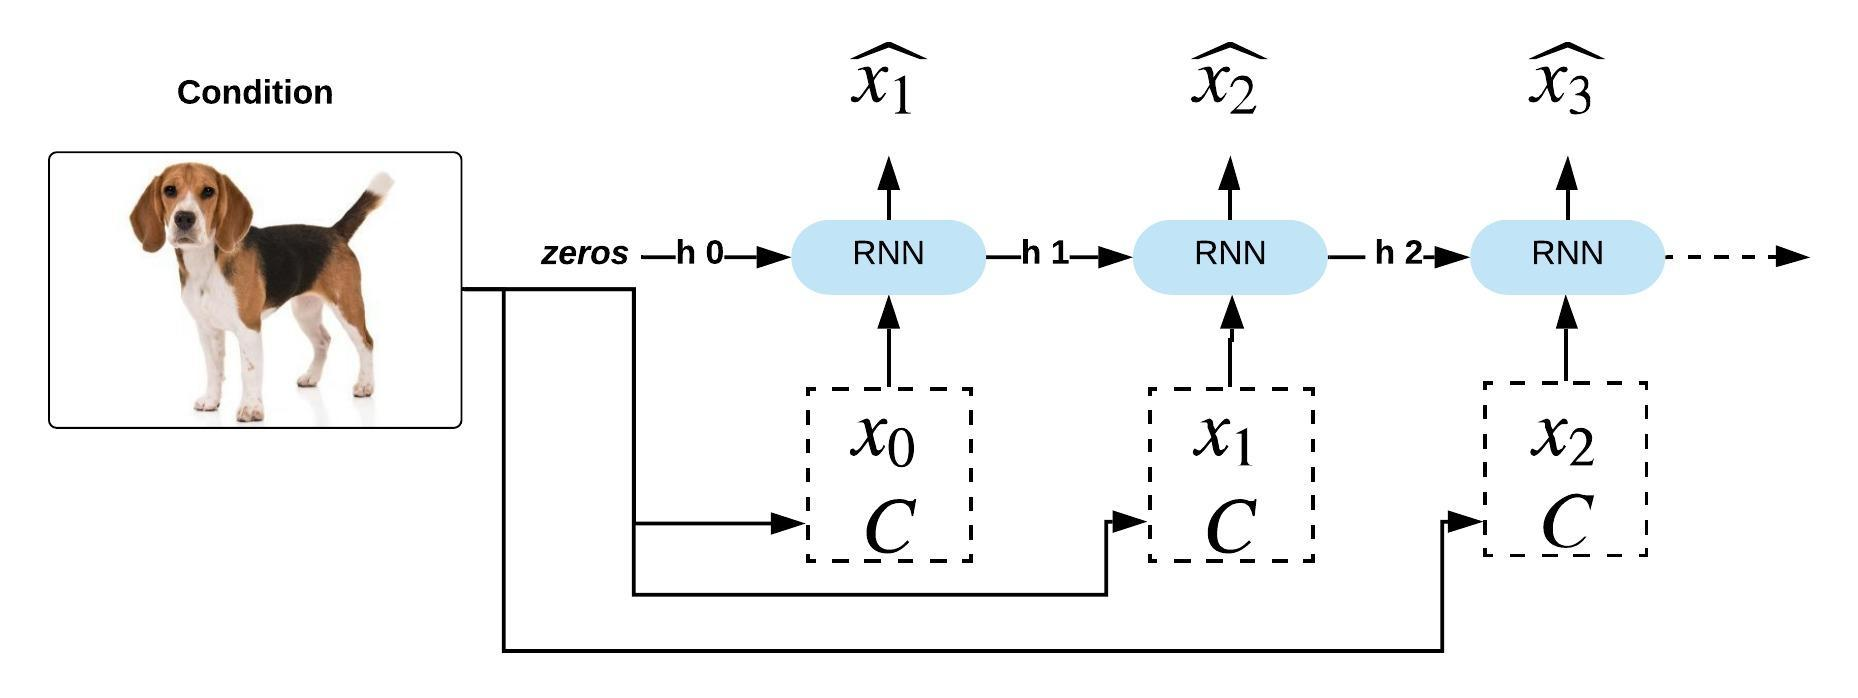
\includegraphics[width=\textwidth]{images/gbem/conditioning_model/cat_timestep.jpeg}
        \caption{Concatenating the condition with time-step, similar to the one used in~\citep{ha2017neural}.}}
        \label{subfig:cat_timestep}
    \end{subfigure}
    \caption{Different conditioning method for RNN}
    \label{fig:conditioning_model}
\end{figure}

\subsection{How to evaluate the quality of generation?}\label{sec:eval_metrics}
  % \OSM{INCOMPLETE SUB-SECTION}
  %
  % \textbf{NOTE: Explore this problem in speech and statistical machine translation/text generation.}
  % \begin{itemize}
  %     \item divide into sections: static and temporal data
  %     \item text, speech evaluation
  %     \item using an oracle model (the error concatenation problem, and the adversarial attack).
  % \end{itemize}
  % \par The problem of evaluating the quality of the generation/synthesis process is a challenging task in the domain of generative models.
  \par The objective evaluation of a generative model is a challenging task, since there is no consensus for objective evaluation metrics. We can not simply make strict comparisons between the generated data and the ground truth, since, as we saw earlier in the inference section, there is asymmetry between the training and the generation task. While a subjective evaluation can be a workaround to this problem, it is quite slow, expensive and hinders the development of new models and approaches. The need for objective evaluation that are consistent with the relevant subjective evaluation is thus a necessity.

  \par Let's see how this problem is approached in different domains:
  % In many cases, a subjective evaluation is performed to overcome this problem. For handwriting of Chinese letters, \cite{DBLP:journals/corr/abs-1801-08624} proposed two metrics:
  \begin{description}
    \item [Text] Evaluating text is an essential task to assess the quality of generation in many applications, like image captioning, language translation and language modeling. An example for an objective text evaluation metric is \textit{BLEU score}~\citep{papineni2002bleu}, which stands for \textit{bilingual evaluation understudy}, it is a well known metric to evaluate text generation applications, like image captioning~\citep{karpathy2015deep,vinyals2015show} and machine translation~\citep{Sutskever:2014:SSL:2969033.2969173}. It tries to capture the human evaluation criteria for the quality of the generated text. It compares individual generated segments -- the size of the segments is a parameter to set -- to see if they exist in the ground truth. It does not focus on the location of that segment, just the fact if it exists or not. The small segments -- letters or words -- are used in order to measure the \textit{adequacy} of the generation, while the longer segments are used to measure the \textit{fluency} of the generation. Usually, the metrics is reported on segments from one to four words, to give and overall idea about the quality of the system.

    Other objective metrics were developed and commonly used, such as \textit{METEOR}~\citep{denkowski:lavie:meteor-wmt:2014} and \textit{Word Error Rate}~\citep{klakow2002testing}.

    \item [Speech synthesis] We are not aware of commonly used objective metrics in this area. A commonly used subjective criteria is Mean opinion score (MOS), which is the average of individuals' opinions on the quality of the system. As an example, the \textit{Blizzard Challenge}~\citep{blizzard} is an annual competition in speech synthesis, to encourage the development of better speech synthesizers. The evaluation is much more detailed that MOS, by trying to assess multiple levels for speech, like intelligibility, naturalness, utterance and the efficiency of the speech. Another evaluation metric used is \textit{MUltiple Stimuli with Hidden Reference and Anchor} (MUSHRA), which uses anchors in order to set a relative reference for the participants to perform the evaluation.

    \item [Handwriting of offline Chinese letters] \cite{DBLP:journals/corr/abs-1801-08624} proposed two metrics to evaluate the quality of their generated letters: content accuracy and style discrepancy. For the first metrics, they train an \textit{evaluator} model on the ground truth data, and use it to recognize the letters produced by their generator. For the second metric, they follow an approach developed in \cite{DBLP:journals/corr/GatysEB15}, where the authors studied the problem of image style transfer, by measuring the correlation between different filter activations (in convolution neural network) at one layer, which represents the style representation.
  \end{description}

  \par We would like to phrase the objective from these metrics here as \textit{the desire to capture the distance between the generated and the ground truth distribution}. It is not important if some individual mistakes happens in the generated sequence, what matters is to capture the essence of the ground truth distribution. That being said, for complex distribution, capturing the distribution, or even measuring the distance between two distributions, is not always a tractable task. As noted in the speech synthesis point, sometimes it is better and more practical to consider multiple criteria in the same time in order to better understand and evaluate the behavior of the system. This point will later reflect our decisions concerning the evaluation  criteria for our work.

  \par Another way to perform the evaluation seen in the literature -- like in~\citep{wang2018style} -- is to use a machine learning model (sometimes called the \textit{Oracle}), trained on the task needed (recognizing the speaker in the synthesized sound for example). In that case, the model is trained on the ground truth, and used in order to evaluate the samples generated by the model. To put simply, we strictly disagree with such approach, for two reasons:
  \begin{description}
    \item [Improper data distribution] It violates the rules of machine learning: if the model is trained on some distribution, then we expect it to perform well on that distribution. What another model generates is simply a different distribution from the ground truth (even though we want this distance to be as close as possible). Thus, the model behavior in this case is not covered in the statistical learning theory. If the oracle -- on the ground truth -- has an accuracy of 90\%, and then we change the data distribution, we can not really trust the prediction of the system, it is no longer the 90\% percent, and we do not know what it is.

    The problem continues when we have two generators, and we want to determine which is best, using an oracle, then we can not really compare them. If one generator achieves 80\% and the other is 85\% accuracy, we can not make a conclusion about which is better. The process itself is flawed. Besides, we do not have access to confidence level on the quality of the oracle, thus it is not possible to perform such comparison using the oracle.

    \item [Adversarial problem] The problem gets worse when we use the oracle in order to evaluate the generator, then use this value as feedback to the generator in order to "improve" it. We experimented on this part to better understand it. Check appendix \ref{ch:adv_eval} for more details.
  \end{description}
  \par The takeaway messages is: it is not about numbers and face value. It is about what these numbers actually means and implies. A model is an approximation of ground truth distribution, and not the ground truth in itself. Thus, dealing with it as the ground truth will easily lead to a loss.
  % \begin{description}
  %     \item[Content accuracy]: They train an \textit{evaluator} model on the ground truth data, and use it to recognize the letters produced by their generator. This approach however faces important problems: the model is trained with ground truth data, and this results in error in the classification, $E_{eval-ref}$. We call the error of the generator $E_{gen}$. When the evaluator is exposed to the data coming from the generator, a new source/distribution of errors is now coming from the generator, which the evaluator have never been exposed to before, leading to a change in the evaluator error behavior. We call this new error $E_{eval-gen}$. Thus, there are no guarantee that the result of the evaluator is faithful in this case. It is also not possible to deduce $E_{gen}$ from just knowing $E_{eval-ref}$ and $E_{eval-gen}$, since the model performance in this case is unknown.
  %     \item[Style discrepancy]: In \cite{DBLP:journals/corr/GatysEB15a}, the authors performed image style transfer: take an image, and transform it to the style of an artist. In order to evaluate the quality of the transfer, they measured the correlation between different filter activations (in convolution neural network) at one layer -- which represents the style representation --. While this metric is interesting to explore, it is not directly applicable to our case, since it assumes the use of convolution neural network.
  % \end{description}
  %
  % \par \cite{mohammed2018DTL} also addressed the problem of evaluation of handwriting generation. They used the \textit{BLEU score} \cite{papineni2002bleu} (a metric widely used in text translation and image captioning) and the \textit{End of Sequence} (EoS) analysis. They showed that these metrics correlate with the quality of the generated letter.
  %
  % \par The BLEU score is global: all frames of the generated sequence contribute to the final score. The BLEU score is used to compare segments of generated traces with the ground truth. Depending on the number of \textit{grams} chosen, the BLEU score can compare larger segments, thus giving us different levels of granularity to assess the quality of the generated samples.

  % The EoS is a simple yet important style feature. Some letters take longer (i.e. written using many strokes, like H or E) to write than other letters (e.g with one stroke like O or C). It is also an idiosyncratic feature of the writer: writers have different writing speeds, depending on age, education or cognitive/peripheral disorders. We used these metrics in our work as well as a letter-specific metric (applicable only to a subset of the data): the average angular momentum of the letter X will be discussed in detail in the section~\ref{sec:evaluation} below.

  % \par The EoS is a simple yet important style feature. Some letters take longer (e.g., written using many strokes, like H or E) to write than other letters (e.g., written with one stroke like O or C). It is also an idiosyncratic feature of the writer: writers have different writing speeds, depending on age, education or cognitive/peripheral disorders.

\section{Putting it all together}
\par In the previous section, we explored multiple building blocks for the work to come, like recurrent neural networks (architectures, training, inference and conditioning). We also discussed the issue of evaluation the output of generative models, discussing three aspects: evaluation in case of text (image captioning, translation, and text generation in general), speech synthesis, and the dangers of using another model (oracle model) in order to evaluate the generation quality.

\par In this section, we discuss how to put all these elements together, the decisions made, and the experimental setup used, in order to address the following three questions:
\begin{itemize}
    \item How to generate handwritten letters using deep learning framework?
    \item How to evaluate the generated traces?
    \item What benchmarks are suitable to compare to?
\end{itemize}

\par Our contributions will be on how to evaluate the generated traces, proposing multiple benchmarks, and using the prior knowledge about the power of those benchmarks in order to ground the the proposed evaluation metrics. The work done in this chapter was published in~\citep{mohammed2018handwriting}.

\subsection{Our proposed evaluation metrics}\label{subsec:eval_metrics}
\par Evaluation is a challenging problem when using generative models. We want metrics to capture the distance between the generated and the ground truth distributions. One of our contributions is to propose using the following metrics:

\paragraph{BLEU score} As mentioned earlier, BLEU score is used in the evaluation of text generation. Since we discretized the letter drawings, this fits nicely within our work. The general intuition is the following: if we take a segment from the generated letter, did this segment happen in the ground truth letter? We keep doing this for segments of increasing length (the length of the segment here is the number of grams used in the BLEU score). For our work, we report the results on segments from 1 to 3 time steps.

Each part of the letter has two parallel segments: freeman codes and speed, thus, we report the BLEU score for both of them.
The equation to compute the BLEU score is the following:
\begin{equation}
BLEU_{N} = \frac{\sum_{C\in G}\sum_{N\in C}Count_{Clipped}(N)}{\sum_{C\in G}\sum_{N\in C}Count(N)}
\end{equation}
\begin{equation}
Score_{N} = \min{(0, 1 - \frac{L_{R}}{L_{G}})} \prod^{N}_{n=1}BLEU_{n}
\end{equation}

where: $G$ is all the generated sequences, $N$ is the total number of N-grams we want to consider. $Count_{Clipped}$ is clipped N-grams count (if the number of N-grams in the generate sequence is larger than the reference sequence, the count is limited to the number in the reference sequence only), $L_R$ is the length of the reference sequence, $L_G$ is the length of the generated sequence. The term $\min(0, 1 - \frac{L_{R}}{L_{G}})$ is added in order to penalize short generated sequences (shorter than the reference sequence), which will deceptively achieve high scores.

\par In order to get into the intuition of using such a metric in evaluating the quality of handwriting generation, we can imagine that we are comparing segments of a generated trace to segments in the ground truth letter, by asking the following question: does the segment in the generated trace exist (anywhere) in the original trace? The shorter segments represent \textit{adequacy} (i.e., does the generated trace use the same elementary moves like the ground truth trace). The longer segments represents \textit{fluency} of drawing (i.e., how good the drawing is)\footnote{This last interpretation of short and long segments is adapted from the~\citep{papineni2002bleu}, which uses them for text translation evaluation.}. See figure~\ref{fig:bleu_score}. Usually, in case of text evaluation, the values of N between 1 and 4 grams are reported. In our work, we report till 3 grams.

\begin{figure}[!htbp]
    \centering
    \begin{subfigure}{0.3\textwidth}
        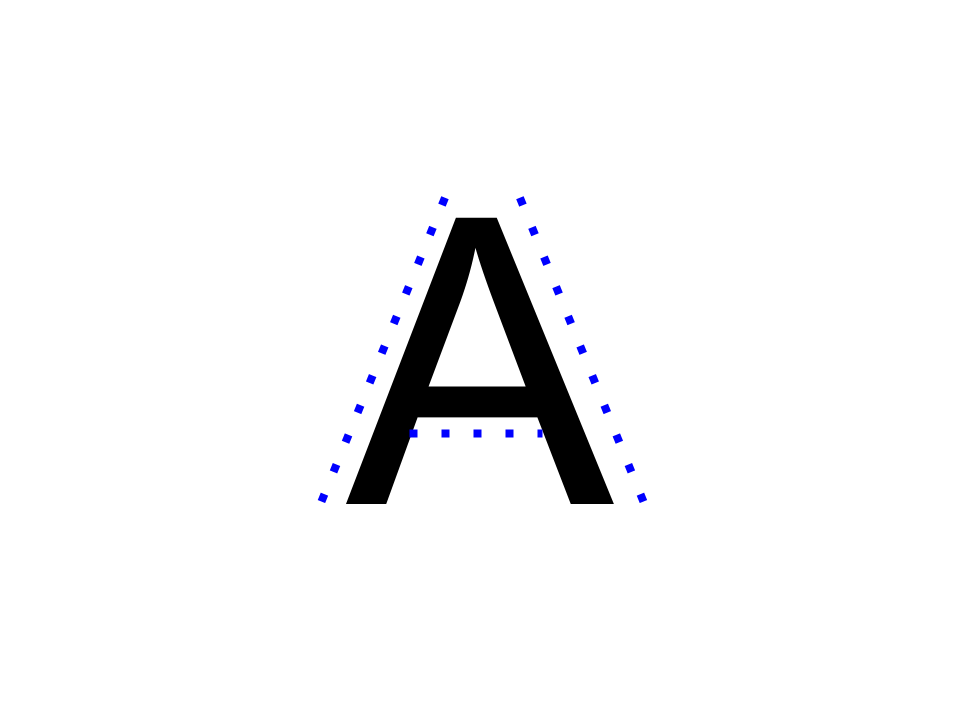
\includegraphics[scale=0.3, trim={10cm 7cm 10cm 7cm},clip]{images/gbem/bleu_score_1.png}
    \end{subfigure}
    ~
    \begin{subfigure}{0.3\textwidth}
        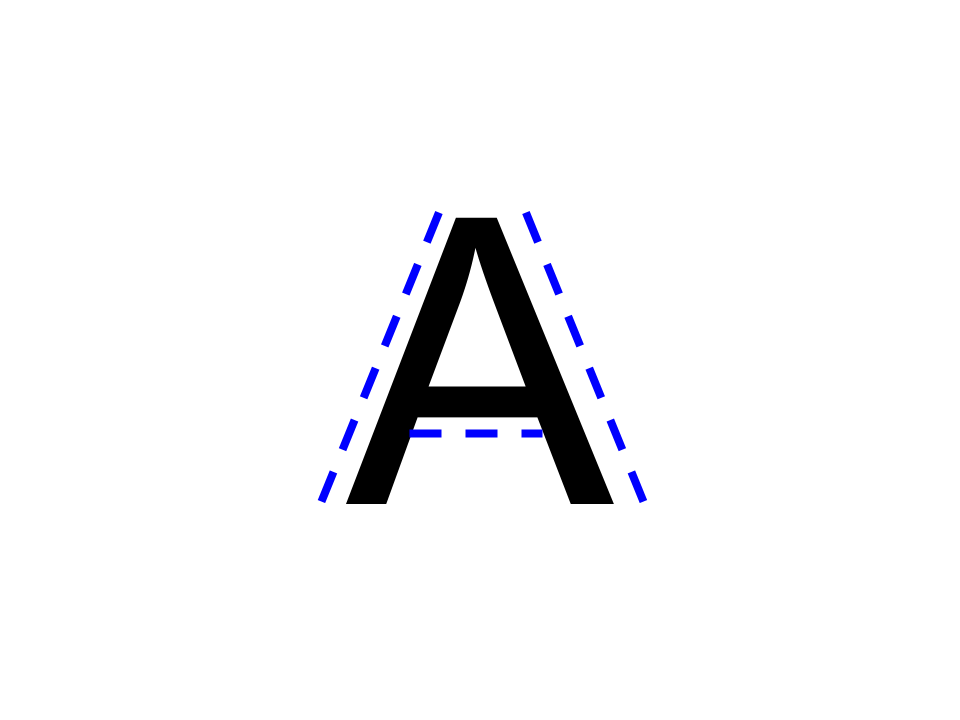
\includegraphics[scale=0.3, trim={10cm 7cm 10cm 7cm},clip]{images/gbem/bleu_score_2.png}
    \end{subfigure}
    ~
    \begin{subfigure}{0.3\textwidth}
        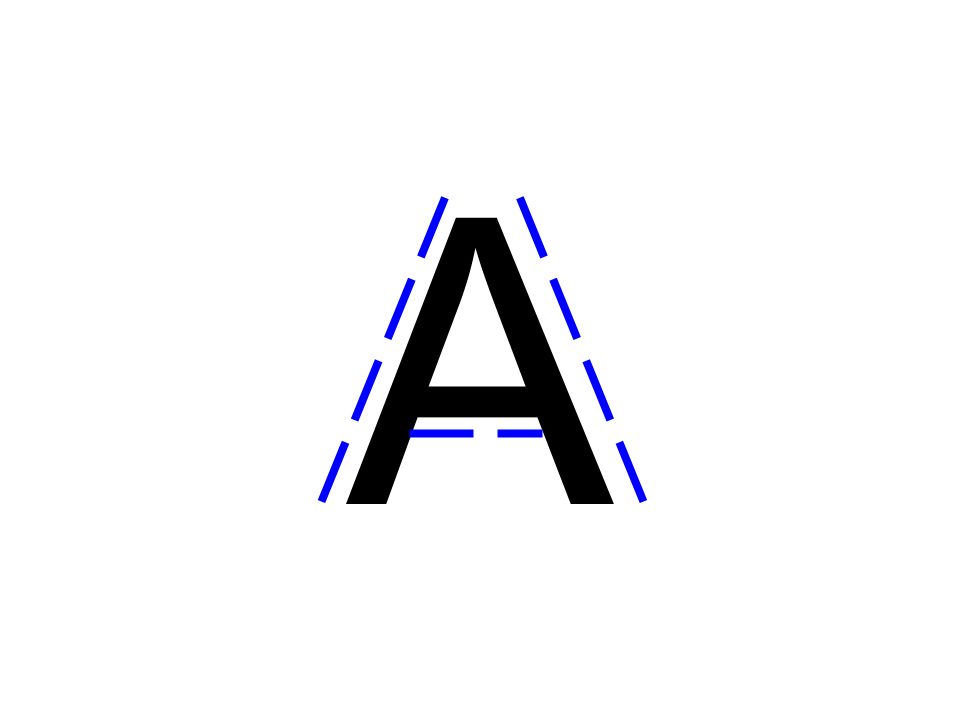
\includegraphics[scale=0.3, trim={10cm 7cm 10cm 7cm},clip]{images/gbem/bleu_score_3.png}
    \end{subfigure}

    \caption{Using BLEU score of different sizes, we compare segments of variable length in the generated trace to the target trace. The smaller BLEU scores evaluate the \texit{adequacy} of the drawing, while the bigger BLEU scores evalute the \textit{fluency}~\citep{papineni2002bleu}.}
    \label{fig:bleu_score}
\end{figure}

\paragraph{End of Sequence} The length of the letter is another aspect of the style. The distribution of length in the generated examples should follow the ground truth examples. In order to perform this analysis, we compute ~\textit{Pearson correlation coefficient} between the generated examples and the ground truth data.

\subsection{How to ground the metrics?}\label{subsec:ground_metrics}
\par We assess multiple methods to condition our handwritten letter generator, and evaluate their ability to capture of writing styles. We know their cardinal order of the power of these methods (depends on the kind of information available to each method). Knowing this information beforehand, we can use it to ground our performance metrics. The methods are:
\begin{description}
    \item[Letter identity]: the letter id only is used as bias. No style information is thus included. The model will try to average over the different example for the same letter. We consider this as a lower baseline.
    \item[Letter + Writer identities]: the letter id and writer id are used as a bias. Thus, the model has an explicit access information about the writer. This method is expected to perform the best. This model will also serve as a upper baseline.
% \end{description}
% \par Starting from the images of the letters, we wanted to test if we can extract information about the style. We two approaches, based on deep learning framework:
% \begin{description}[noitemsep]
    \item[Image classifier embedding]: we train a convolution neural network (CNN) to classify the letters images\footnote{This letter classification task achieves $95.1\%$ classification accuracy, which we consider very good.}, as shown in figure~\ref{fig:architectures}. We use an intermediate layer as to extract embeddings, that will encode information about the letter images. This model should perform the same or a more performance than using the letter identity only, since it learns to clusters the letters, and there are classification errors. But we expect it to perform less than the letter + writer identities.
    \item[Image auto-encoder latent space]: we train a letter image autoencoder, using reconstruction error, and use the latent space as a representation of the letter + style. The architecture we use can be seen in figure~\ref{fig:architectures}. The latent space encodes the similarity between the letters. This model should perform worse than using the letter identity only, since, while it capture the similarity between the letter images, it does not capture discriminative features about each letter itself.
\end{description}

\par From this discussion, we can say that cardinal power of the different conditions is:
% \begin{subequations}
\begin{align}
    & autoencoder < letter \leq classifier < letter+writer
    \label{eq:cardinal_power}
\end{align}
% \end{subequations}

\begin{figure}[!htbp]
    \centering
    \begin{subfigure}{0.4\textwidth}
        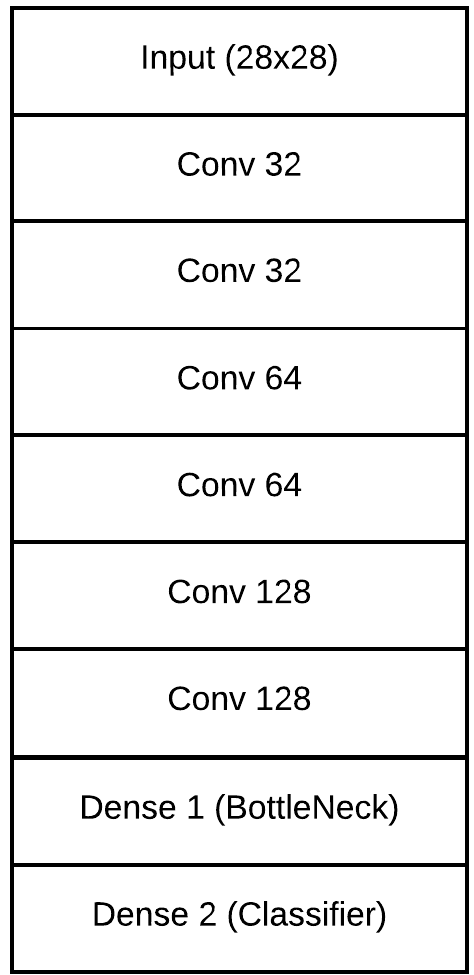
\includegraphics[scale=1.0]{images/gbem/classifier.png}
    \end{subfigure}
    ~
    \begin{subfigure}{0.4\textwidth}
        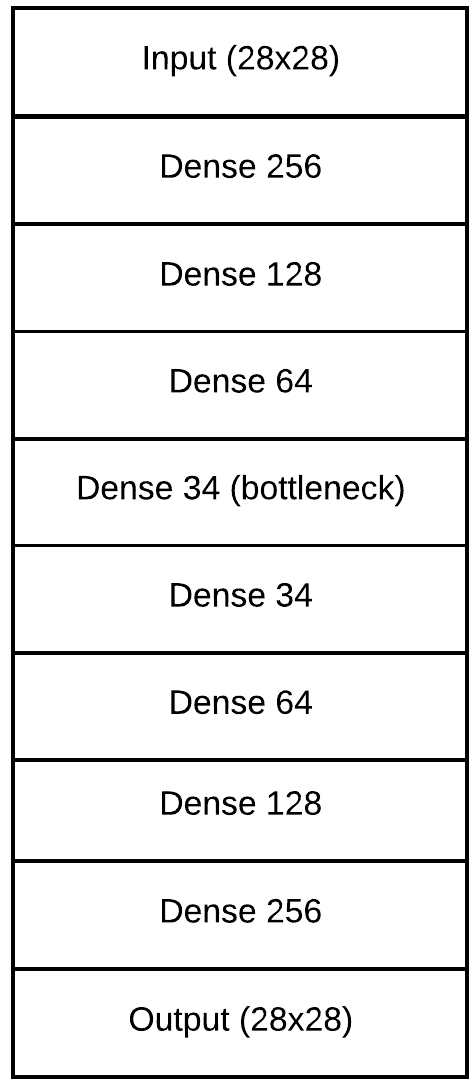
\includegraphics[scale=1.0]{images/gbem/autoenc.png}
    \end{subfigure}
    \caption{Left: architecture of the CNN letter classifier we used. Batch normalization is used after each convolution layer. The \textit{Dense 1} layer -- with a size of 34 -- is the embedding that is used to condition our generator. Right: the autoencoder architecture we used. The output of the first \textit{Dense 34} layer provides the latent space used to condition the generator.}
    \label{fig:architectures}
\end{figure}

\subsection{Proposed model}
We use a type of RNN called Gated-Recurrent Network (GRU)~\citep{chung2014empirical}, which is known for having a better memory ability than basic RNN, thus, making it suitable choice for long sequence. Our model is a conditioned-GRU model, demonstrated in figure~\ref{fig:dtl_model}. Using this model, we compare different style approached discussed in section~\ref{subsec:ground_metrics}, and use the generation results from that model in order to ground the proposed evaluation metrics, discussed in section~\ref{subsec:eval_metrics}.
\begin{figure}[!htbp]
    \centering
    \begin{subfigure}[b]{\textwidth}
        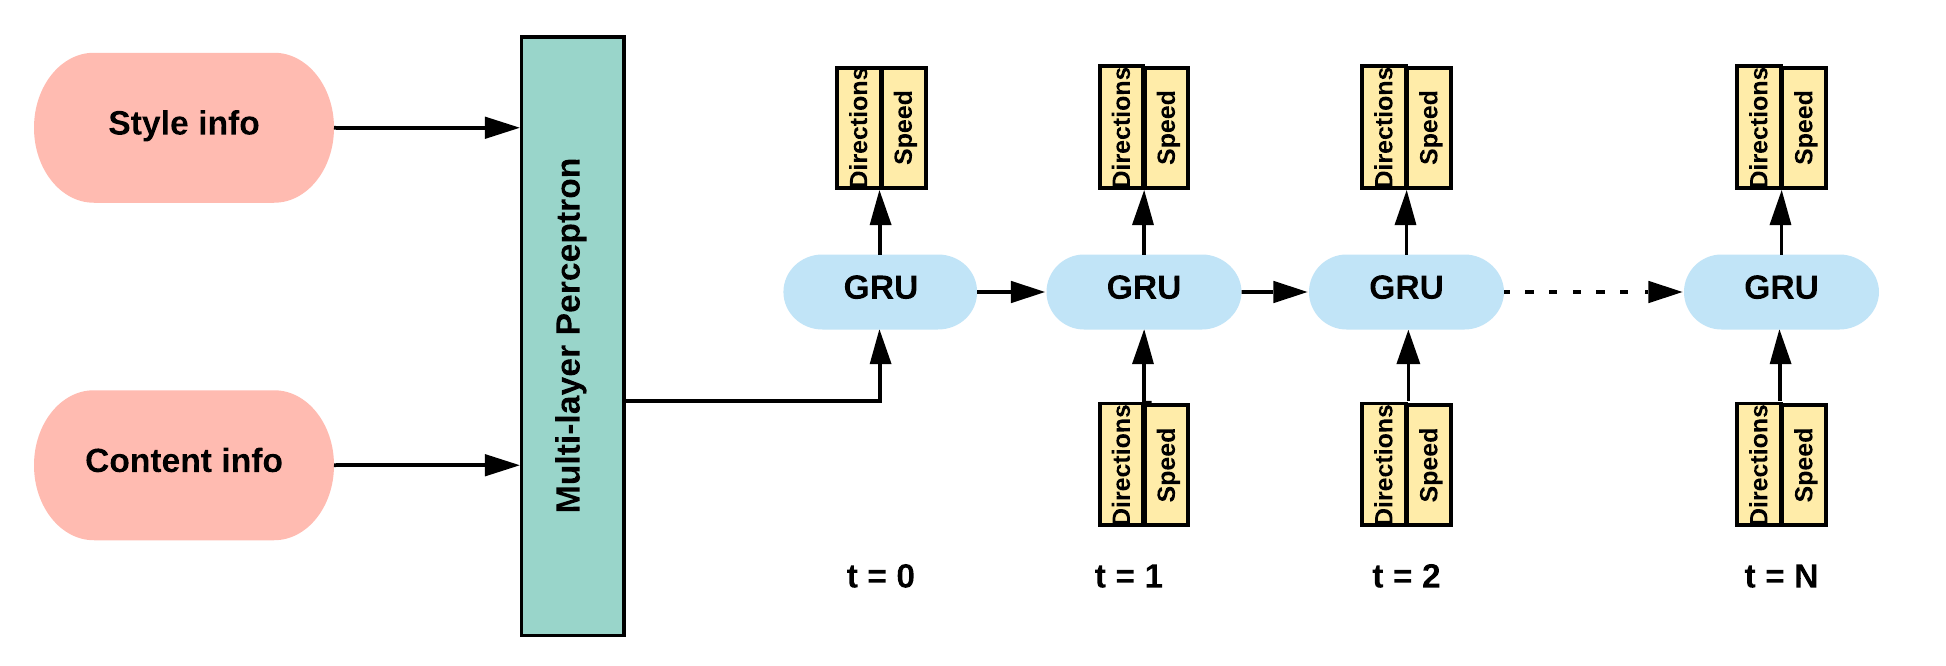
\includegraphics[width=\textwidth]{images/gbem/dtl_training.png}
        \caption{Training mode, using \textit{teacher forcing} methodology~\citep{Williams:1989:LAC:1351124.1351135,Goodfellow-et-al-2016}, where the model gets its input from the ground truth all the time.}
        \label{subfig:dtl_training}
    \end{subfigure}
    ~
    \begin{subfigure}[b]{\textwidth}
        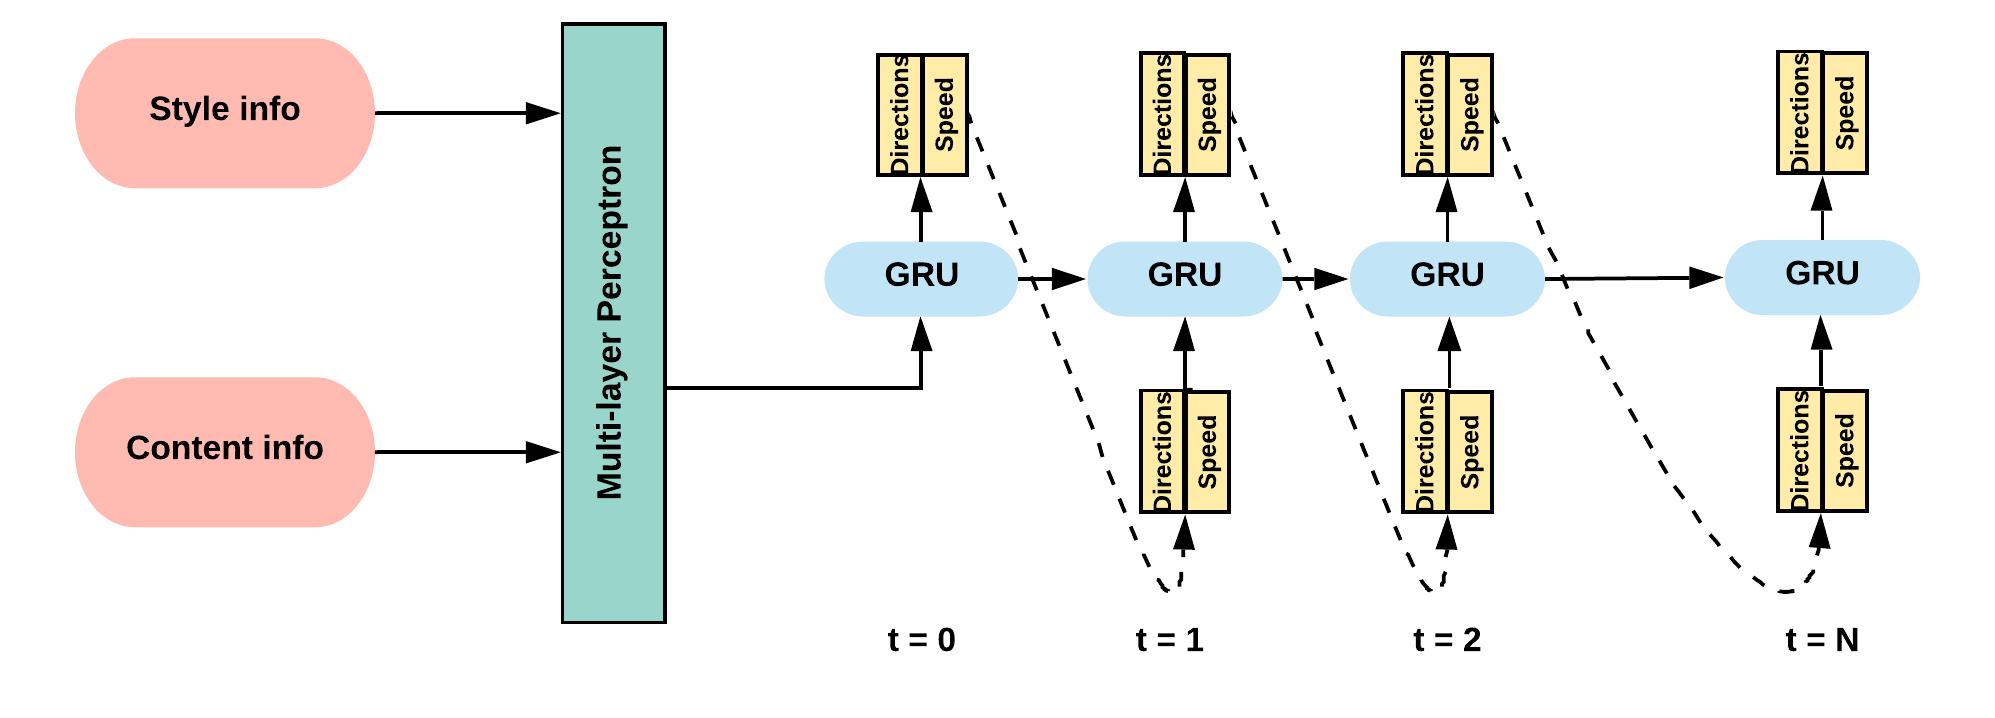
\includegraphics[width=\textwidth]{images/gbem/dtl_generation.png}
        \caption{Generation/Inference mode, where the model gets its input at each time step from its own output at the previous time step.}
        \label{subfig:dtl_generation}
    \end{subfigure}

    \caption{The conditioned-GRU model used in this work. During the training mode~\subref{subfig:dtl_training}, the input of the model is always the ground truth, and the predicted value is compared to the ground truth. During the generation mode~\subref{subfig:dtl_generation}, the input to the model at each step is the model prediction from the previous step. The 'style info' and the 'task info' inputs are separated here for illustration (they could be mixed).}
    \label{fig:dtl_model}
\end{figure}

\par We ran random hyper-parameter tuning over a wide range of parameters, in order to select the final model. The selected model were a based GRU cell, with 3 hidden layers, each of size $256$, and a dropout of $0.3$. Adam optimizer~\citep{kingma2014adam} is selected, with a learning rate of $10^-3$. A \textit{Multi-Layer Perceptron} (MLP) is applied to the output of the GRU at each time step, with an output size of 34. Two SoftMax operation are then applied, in order to extract the freeman code and the speed level.

\subsection{Results}
\par We train our different models and generate the traces from them as explained earlier. In this section, we compare the different models using the evaluation metrics discussed before. We  observe the consistency of the reported metrics with the prior information about the cardinal power of the different methods, equation~\ref{eq:cardinal_power}. This is how we ground our metrics.

\subsubsection{BLEU score}
\par The final results using the BLEU score can be seen in table~\ref{table:1}. The results vary when measuring BLEU-1. But, as we increase the number of grams, BLEU-2 and BLEU-3, to measure the similarity between larger segments of the traces, we can observe:
\begin{itemize}
    \item The letter + writer condition performed better than all other conditions, thus showing that having access to information about the writer, like the writer id, improve the quality of the handwriting synthesis.
    \item The image classifier condition performs better than the letter identity only, but less than the letter + writer bias. Since the classifier is trained on a single objective only (to classify the letters), and the classifier performs well, we expect the embedding to cluster the letters well, as seen in figure~\ref{fig:classifier_autoenc_bottleneck}. We can expect the model to capture some of the writer style, possibly in the inter-cluster variance. This is an interesting result, suggesting that some fine tuning for the image classifier while in the generation task could be beneficial to capture more details about the styles.
    \item The image autoencoder bias performed the worst. To understand why, we plot a 2-D projection of its latent space using t-SNE~\citep{maaten2008visualizing}, figure~\ref{fig:classifier_autoenc_bottleneck}. Since the autoencoder is trained to minimize the reconstruction error, the distance in the latent space encode the proximity between the images. It can be observed also that this latent space does not encode discriminative features for the letters. Using this latent space for our generator, we find the model gets confused between nearby letters, resulting sometimes in generating different letters than requested.
\end{itemize}

\begin{table}[!htbp]
\centering
\begin{tabular}{l|c c c|c c c}
\hline
\multicolumn{1}{c|}{Aspect/Feature} & \multicolumn{3}{c|}{ Speed } & \multicolumn{3}{c}{ Freeman }   \\ \hline
% \hline
Model / B-score      & B-1  & B-2  & B-3           & B-1  & B-2   & B-3              \\ \hline
Letter identity          & 49.7 & 37.3 & 24.2          & 47.4 & 36.6  & 26.8               \\\hline
Image classifier     & 50.9 & 38.2 & 24.6          & 48.5 & 37.9 & 28.1             \\\hline
Image autoencoder    & \textbf{51.9} & 37.9 & 23.1          & 46.4 & 35.0  & 24.5             \\\hline
\textbf{Letter + Writer identities} & 51.5 & \textbf{41.4} & \textbf{25.1}          & \textbf{56.7} & \textbf{39.4}  & \textbf{28.3}             \\\hline
\end{tabular}
\caption{Comparing different approaches for style extraction using clipped n-grams. The higher the value, the better.}
\label{table:1}
\end{table}

\begin{sidewaysfigure}[!htbp]
    \begin{center}
      % ~
      \begin{subfigure}[b]{0.75\textwidth}
        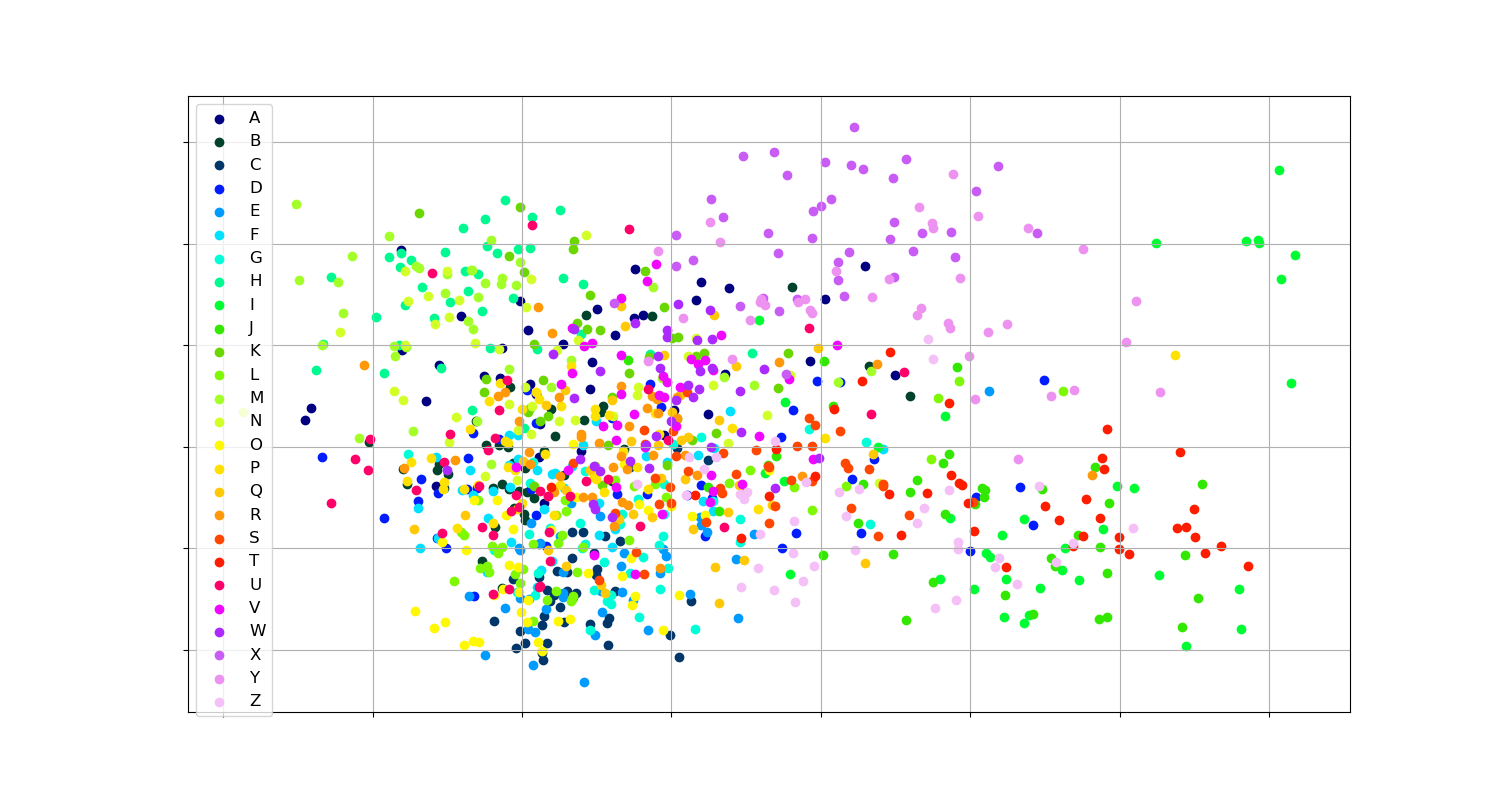
\includegraphics[scale=0.39]{images/gbem/auto_Vis_pca.png}
        \caption{Bottleneck of the auto-encoder}
        \label{subfig:autoenc_latent}
      \end{subfigure}
      \quad
      \begin{subfigure}[b]{0.75\textwidth}
        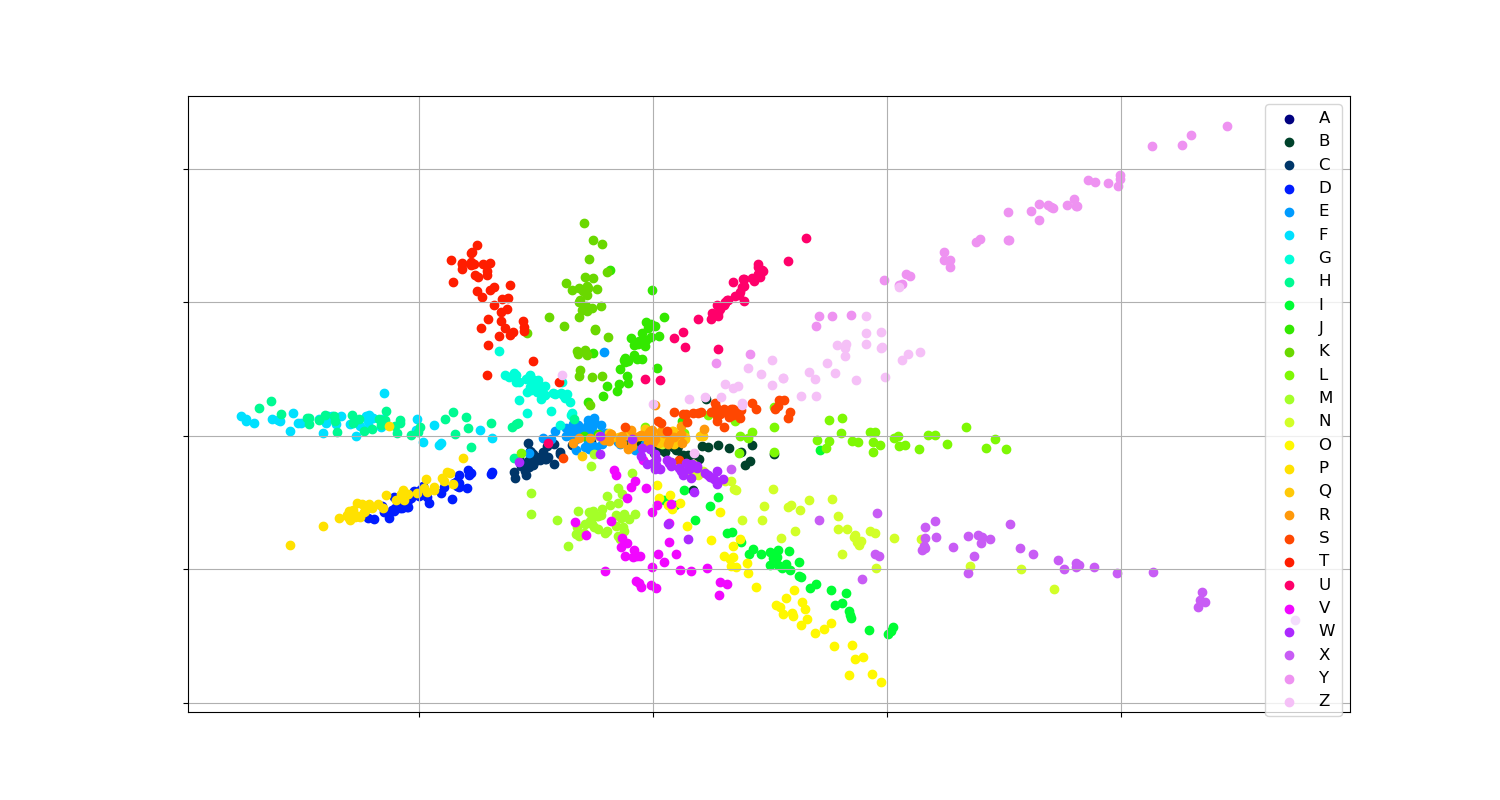
\includegraphics[scale=0.39]{images/gbem/class_Vis_pca.png}
        \caption{Bottleneck of the classifier}
        \label{subfig:classifier_latent}
      \end{subfigure}
      % \caption{Shape of the autoencoder latent space. Left: each color represent one letter. Right: labeling for some of the letters, to illustrate proximity.}
      % 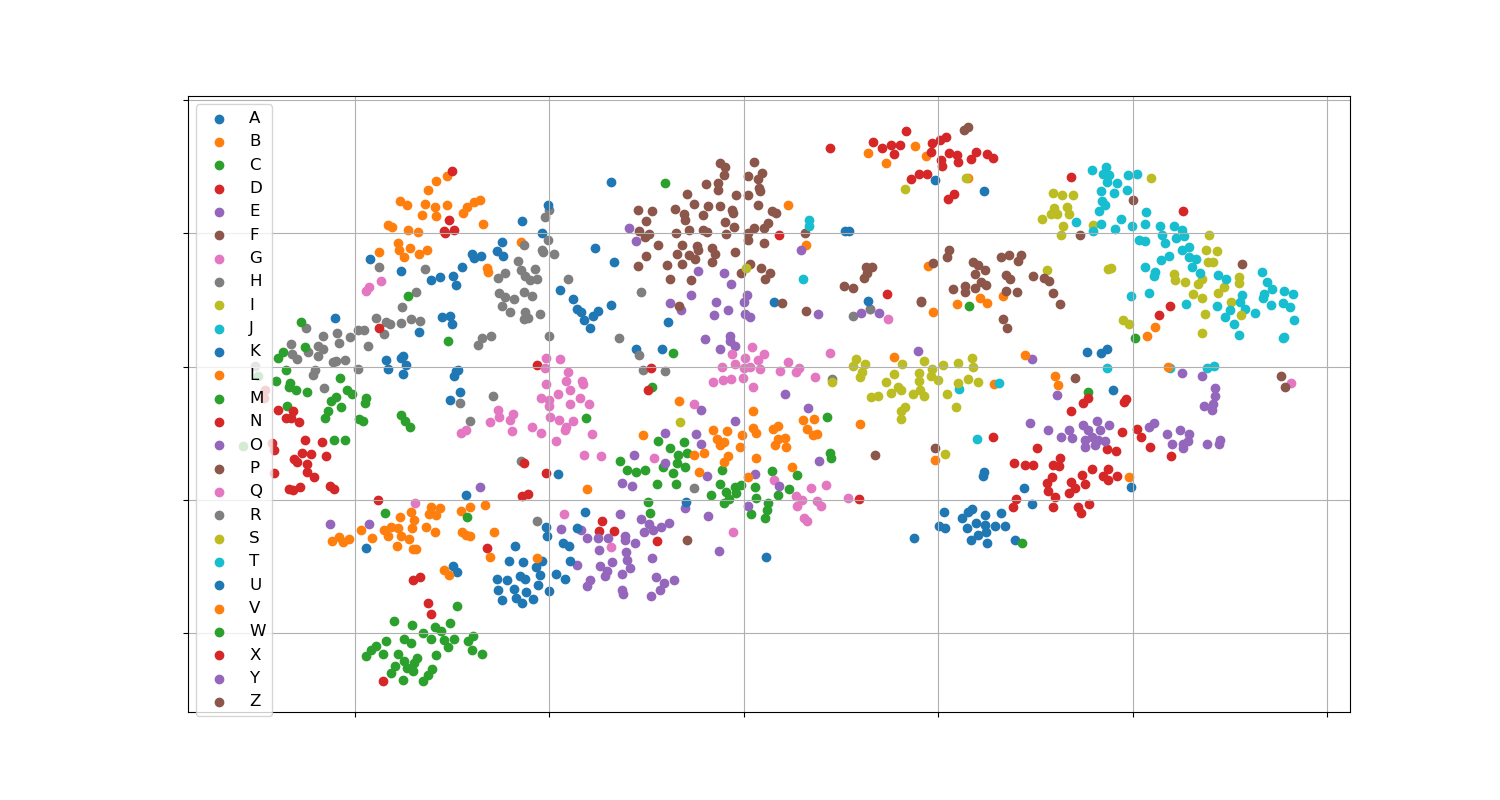
\includegraphics[width=\textwidth]{figures/AutoEnc_Vis_tsne.png}
      \caption{We project the bottlenecks of both the autoencoder and the classifier, using PCA, in order to get an idea about the reason these bottlenecks lead to a very different performance. Figure \subref{subfig:autoenc_latent} shows the autoencoder latent space, there is no clear separation between letters; the encoding is based on the similarity of the images only, while figure \subref{subfig:classifier_latent} shows the classifier embedding, there is a clear separation between the letters - with few exceptions -.}
      \label{fig:classifier_autoenc_bottleneck}
    \end{center}

\end{sidewaysfigure}

\subsubsection{Sequence length}
\par As mentioned earlier, we performed a statistical test between the paired distributions of lengths of the generated and the reference tracings. The results are shown in table~\ref{table:2}. We can see the following:
\begin{itemize}
    \item The results from the statistical test shows that the letter + writer bias outperform the rest of the biases, achieving p-value $< 0.05$. This is quite reassuring, since it is also in line with the results from the BLEU score.
    \item The results from the Pearson correlation coefficients are also consistent with the rest of the results. High coefficients are given to the letter + writer bias, compared to the other methods. The image classifier and autoencoder gives the lowest results. This could be due to insufficient information about the letter length that can be inferred from the image. For the image classifier, as noted earlier, a fine-tuning during the generation task is worth exploring.
\end{itemize}

\begin{table}[!htbp]
\centering
% \begin{tabular}{|c|c|c|}
\begin{tabular}{l c c} \hline
Models & Pearson coefficient & p-value \\ \hline
Letter bias & 0.38 & 0.84 \\ \hline
Image classifier & 0.32 & 0.62\\ \hline
Image autoencoder & 0.25 & 0.29 \\ \hline
\textbf{Letter + Writer bias} & \textbf{0.55} & \textbf{0.04}\\ \hline
\end{tabular}
\caption{Pearson correlation coefficients and associated p-values for the EOS distributions of the different style biases. A \textit{letter + writer} bias performs much better than others biases, while the \textit{image autoencoder} bias performs the worse. This confirms with our expectations about the relative power of the different biases.}

\label{table:2}
\end{table}

\subsection{Examples of the generated letters}
\par The design choices of our experiments (discretization, and ignoring the pen state) affects the final shape of the letters, yet, the letters and their style are quite recognizable. See examples for the original letters in figure~\ref{fig:orig_letters_examples}. Examples for the generation with our methods are in figure~\ref{fig:letters_examples_gbem}. This is a subjective indication that our model is working properly, producing real-like comprehensible letters.

\begin{sidewaysfigure}%[!htbp]
\centering
    \begin{subfigure}[b]{0.14\textwidth}
        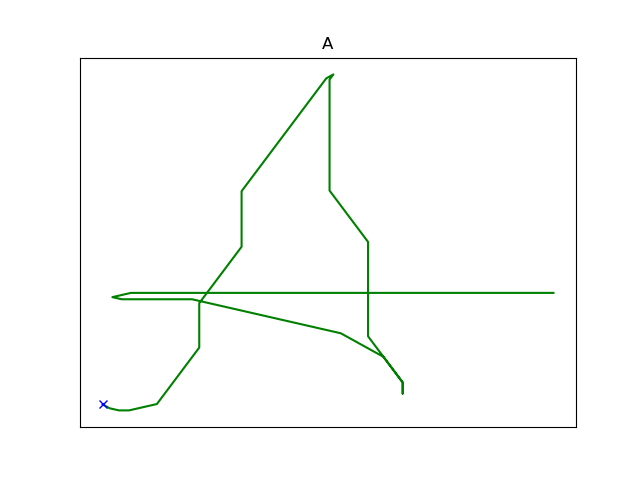
\includegraphics[width=\textwidth]{images/gbem/orig_letters_fig/AORIG_letter_A_writer_8.png}
        \caption{B}
    \end{subfigure}
    ~
    \begin{subfigure}[b]{0.14\textwidth}
        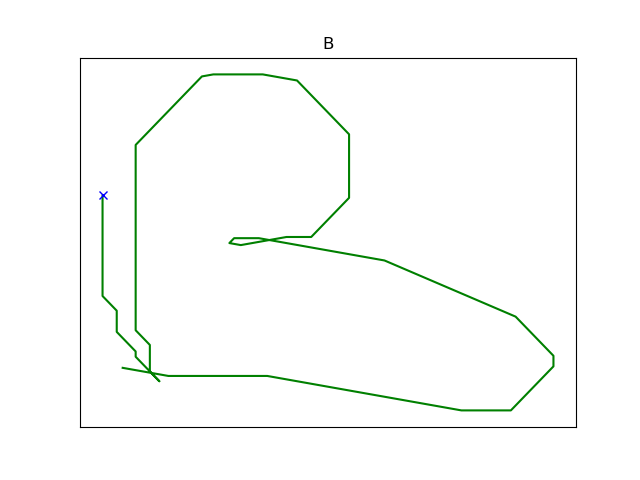
\includegraphics[width=\textwidth]{images/gbem/orig_letters_fig/AORIG_letter_B_writer_7.png}
        \caption{C}
    \end{subfigure}
    ~
    \begin{subfigure}[b]{0.14\textwidth}
        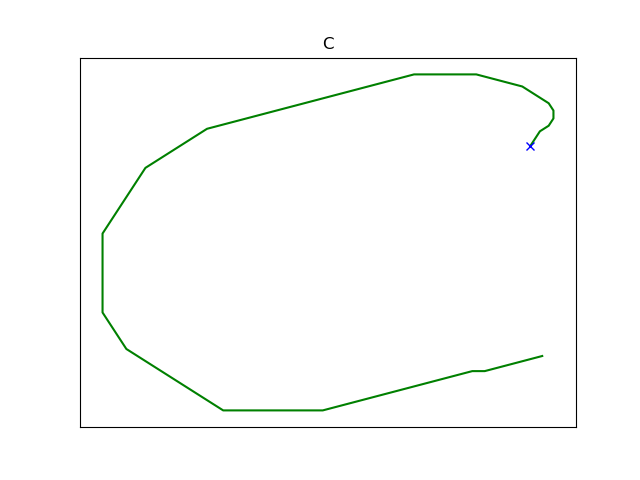
\includegraphics[width=\textwidth]{images/gbem/orig_letters_fig/AORIG_letter_C_writer_5.png}
        \caption{D}
    \end{subfigure}
    ~
    \begin{subfigure}[b]{0.14\textwidth}
        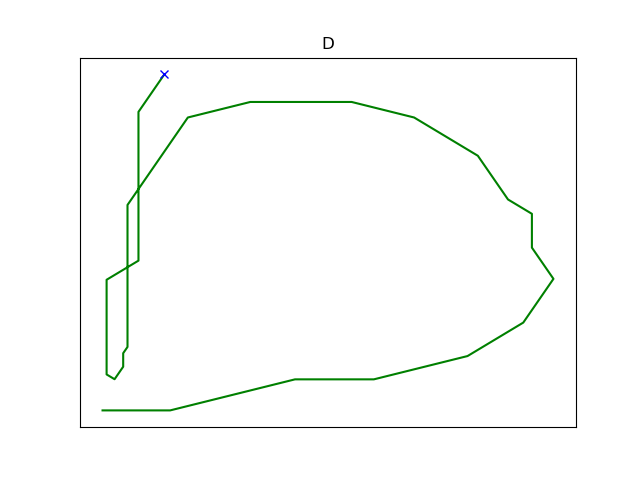
\includegraphics[width=\textwidth]{images/gbem/orig_letters_fig/AORIG_letter_D_writer_6.png}
        \caption{A}
    \end{subfigure}
    ~ %add desired spacing between images, e. g. ~, \quad, \qquad, \hfill etc.
      %(or a blank line to force the subfigure onto a new line)
    \begin{subfigure}[b]{0.14\textwidth}
        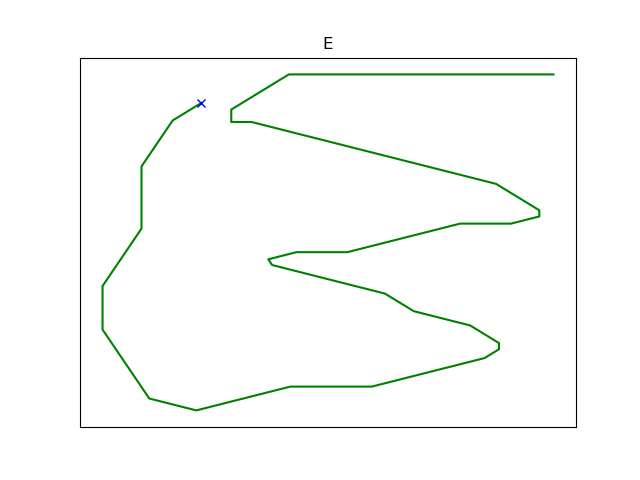
\includegraphics[width=\textwidth]{images/gbem/orig_letters_fig/AORIG_letter_E_writer_6.png}
        \caption{E}
    \end{subfigure}
    ~
    \begin{subfigure}[b]{0.14\textwidth}
        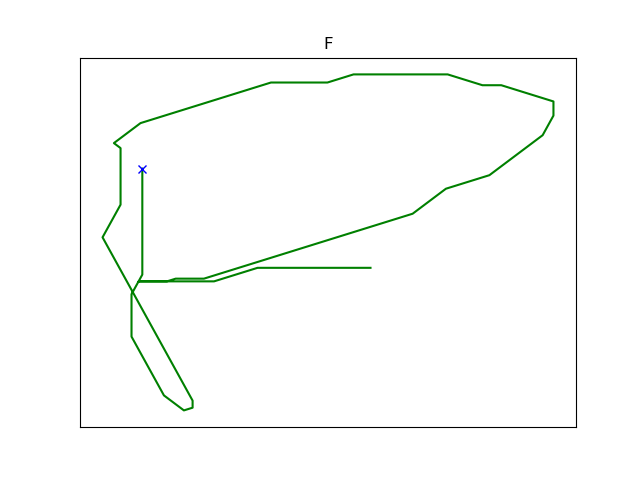
\includegraphics[width=\textwidth]{images/gbem/orig_letters_fig/AORIG_letter_F_writer_4.png}
        \caption{F}
    \end{subfigure}
    ~
    \begin{subfigure}[b]{0.14\textwidth}
        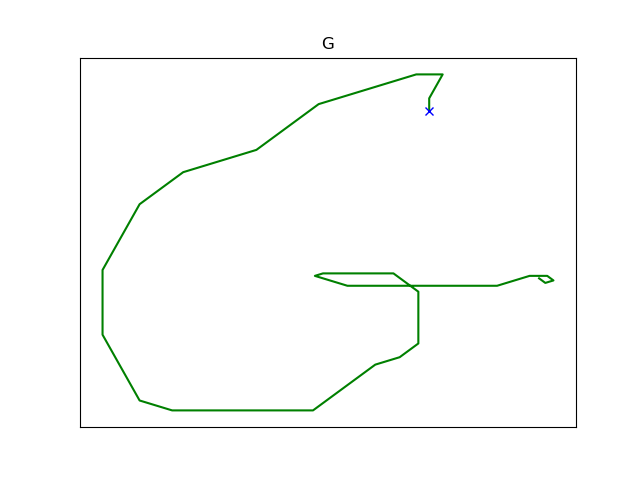
\includegraphics[width=\textwidth]{images/gbem/orig_letters_fig/AORIG_letter_G_writer_5.png}
        \caption{G}
    \end{subfigure}
    ~
    \begin{subfigure}[b]{0.14\textwidth}
        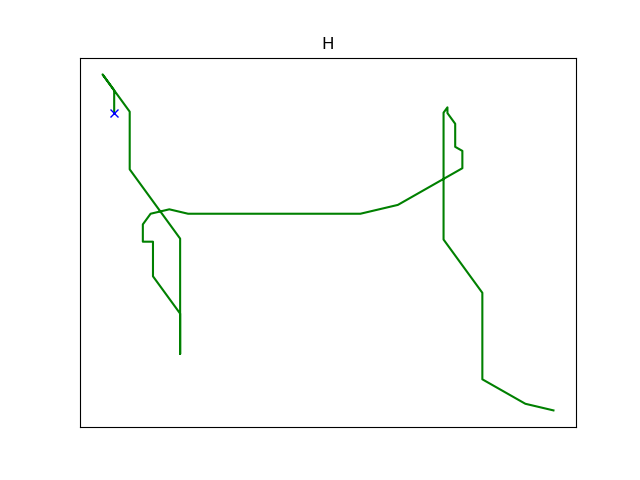
\includegraphics[width=\textwidth]{images/gbem/orig_letters_fig/AORIG_letter_H_writer_16.png}
        \caption{H}
    \end{subfigure}
    ~
    \begin{subfigure}[b]{0.14\textwidth}
        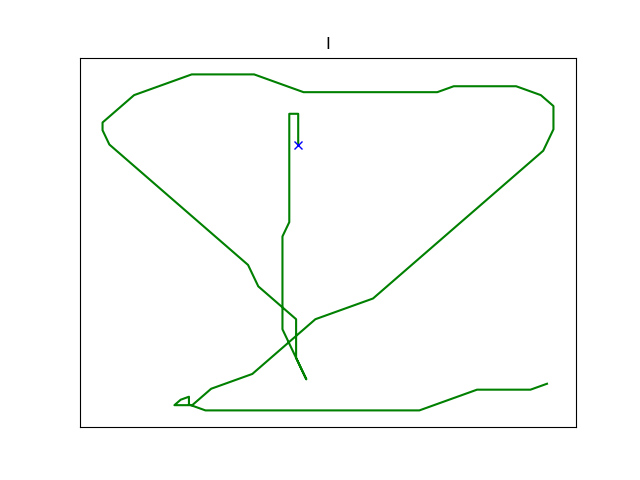
\includegraphics[width=\textwidth]{images/gbem/orig_letters_fig/AORIG_letter_I_writer_5.png}
        \caption{I}
    \end{subfigure}
    ~
    \begin{subfigure}[b]{0.14\textwidth}
        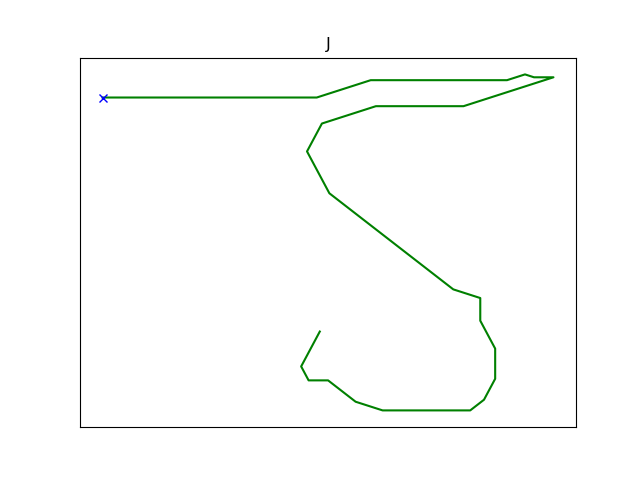
\includegraphics[width=\textwidth]{images/gbem/orig_letters_fig/AORIG_letter_J_writer_4.png}
        \caption{J}
    \end{subfigure}
    ~
    \begin{subfigure}[b]{0.14\textwidth}
        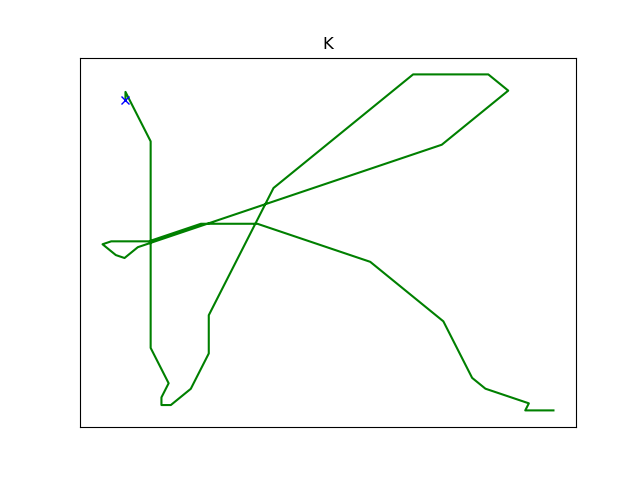
\includegraphics[width=\textwidth]{images/gbem/orig_letters_fig/AORIG_letter_K_writer_4.png}
        \caption{K}
    \end{subfigure}
    ~
    \begin{subfigure}[b]{0.14\textwidth}
        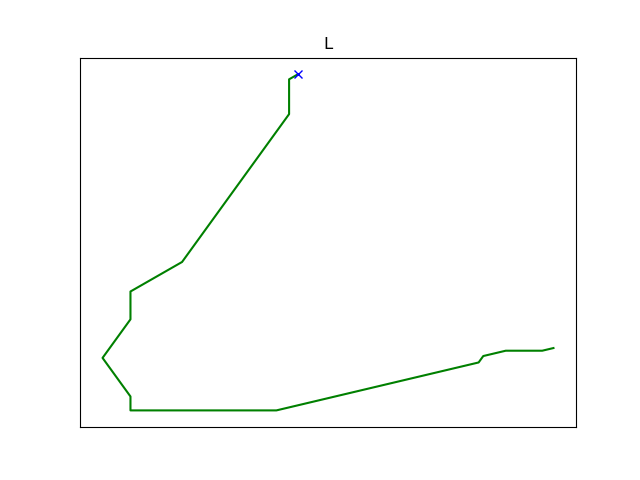
\includegraphics[width=\textwidth]{images/gbem/orig_letters_fig/AORIG_letter_L_writer_16.png}
        \caption{L}
    \end{subfigure}
    ~
    \begin{subfigure}[b]{0.14\textwidth}
        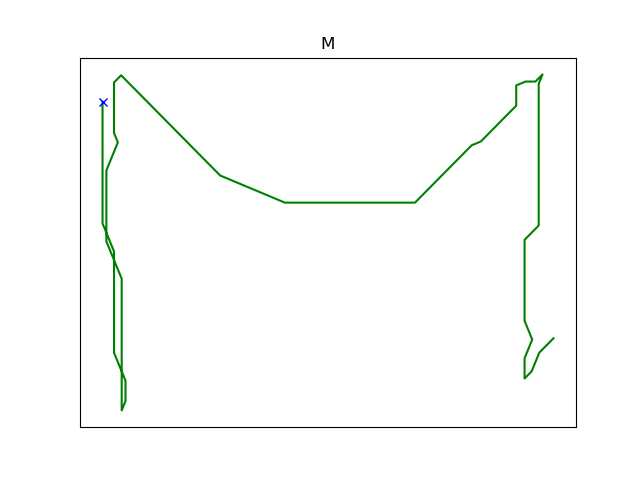
\includegraphics[width=\textwidth]{images/gbem/orig_letters_fig/AORIG_letter_M_writer_10.png}
        \caption{M}
    \end{subfigure}
    ~
    \begin{subfigure}[b]{0.14\textwidth}
        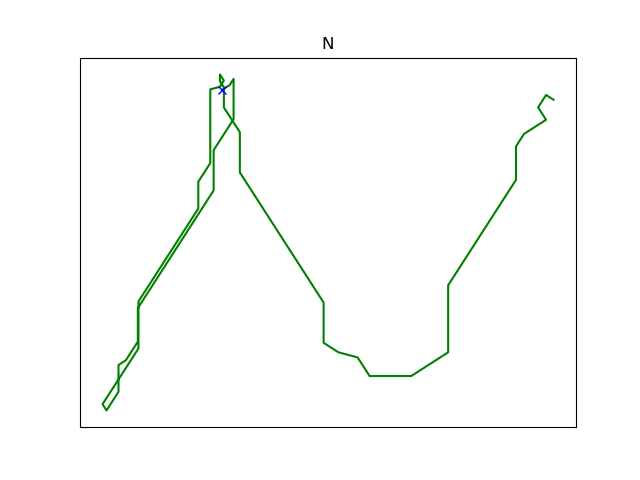
\includegraphics[width=\textwidth]{images/gbem/orig_letters_fig/AORIG_letter_N_writer_1.png}
        \caption{N}
    \end{subfigure}
    ~
    \begin{subfigure}[b]{0.14\textwidth}
        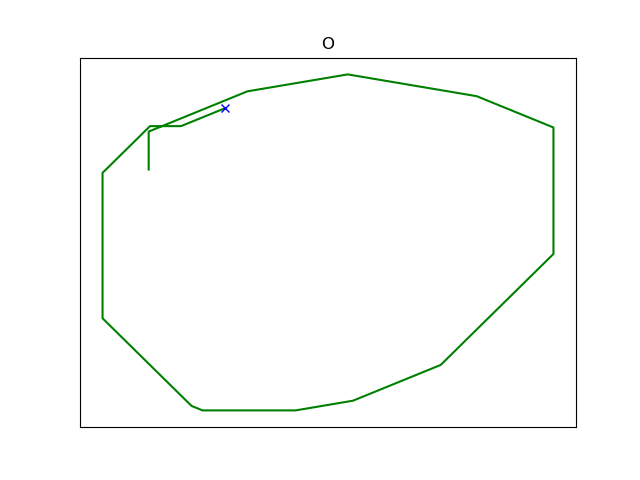
\includegraphics[width=\textwidth]{images/gbem/orig_letters_fig/AORIG_letter_O_writer_2.png}
        \caption{O}
    \end{subfigure}
    ~
    \begin{subfigure}[b]{0.14\textwidth}
        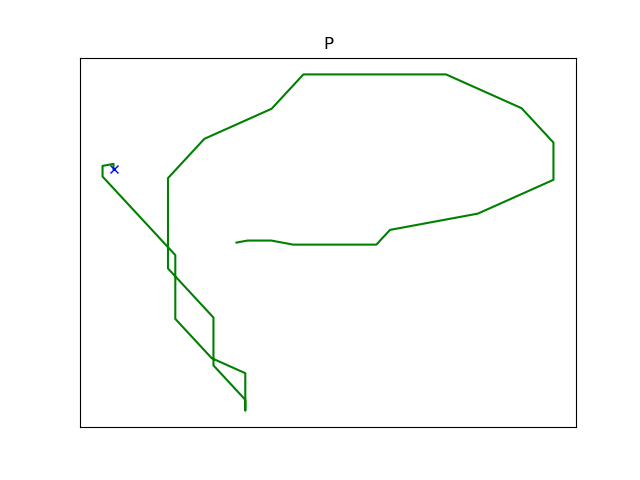
\includegraphics[width=\textwidth]{images/gbem/orig_letters_fig/AORIG_letter_P_writer_11.png}
        \caption{P}
    \end{subfigure}
    ~
    \begin{subfigure}[b]{0.14\textwidth}
        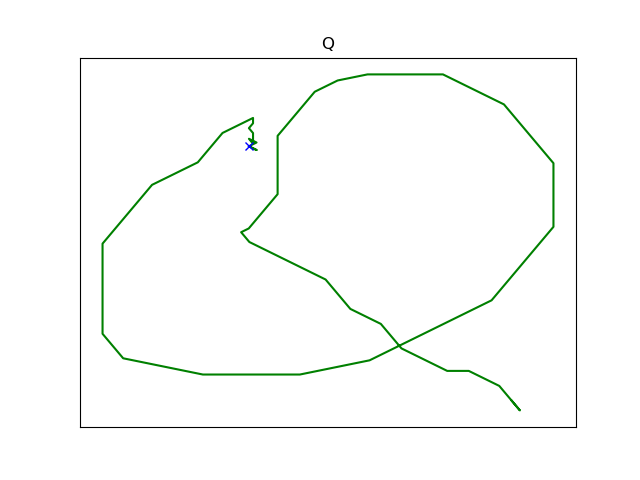
\includegraphics[width=\textwidth]{images/gbem/orig_letters_fig/AORIG_letter_Q_writer_4.png}
        \caption{Q}
    \end{subfigure}
    ~
    \begin{subfigure}[b]{0.14\textwidth}
        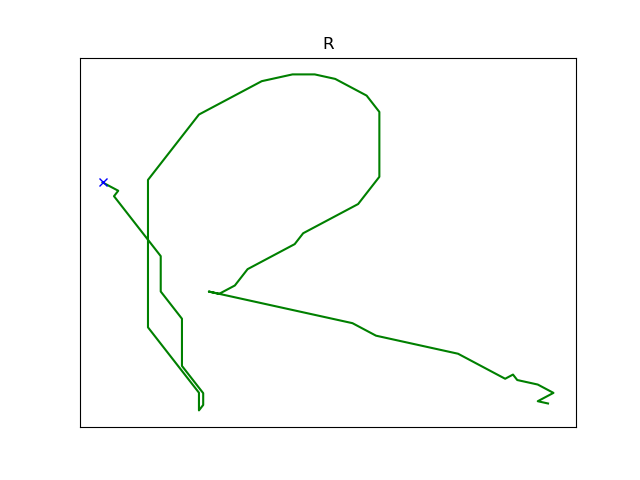
\includegraphics[width=\textwidth]{images/gbem/orig_letters_fig/AORIG_letter_R_writer_2.png}
        \caption{R}
    \end{subfigure}
    ~
    \begin{subfigure}[b]{0.14\textwidth}
        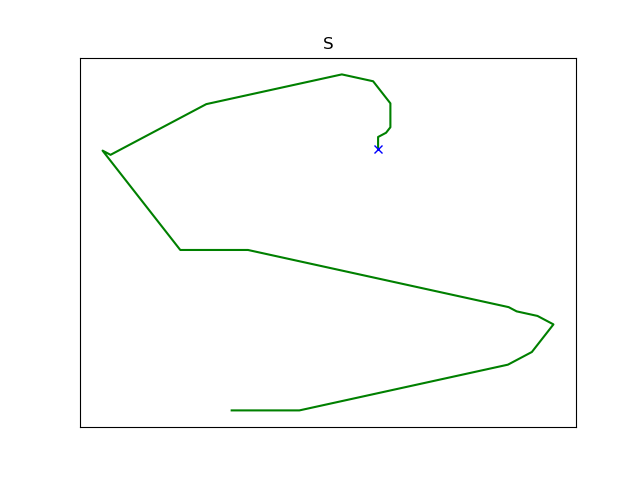
\includegraphics[width=\textwidth]{images/gbem/orig_letters_fig/AORIG_letter_S_writer_1.png}
        \caption{S}
    \end{subfigure}
    ~
    \begin{subfigure}[b]{0.14\textwidth}
        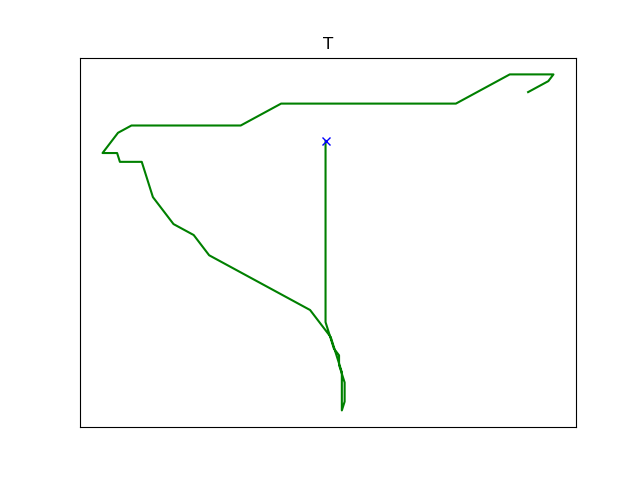
\includegraphics[width=\textwidth]{images/gbem/orig_letters_fig/AORIG_letter_T_writer_1.png}
        \caption{T}
    \end{subfigure}
    ~
    \begin{subfigure}[b]{0.14\textwidth}
        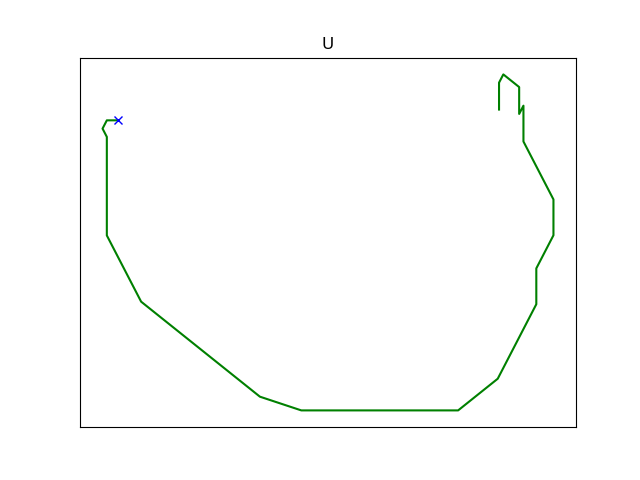
\includegraphics[width=\textwidth]{images/gbem/orig_letters_fig/AORIG_letter_U_writer_5.png}
        \caption{U}
    \end{subfigure}
    ~
    \begin{subfigure}[b]{0.14\textwidth}
        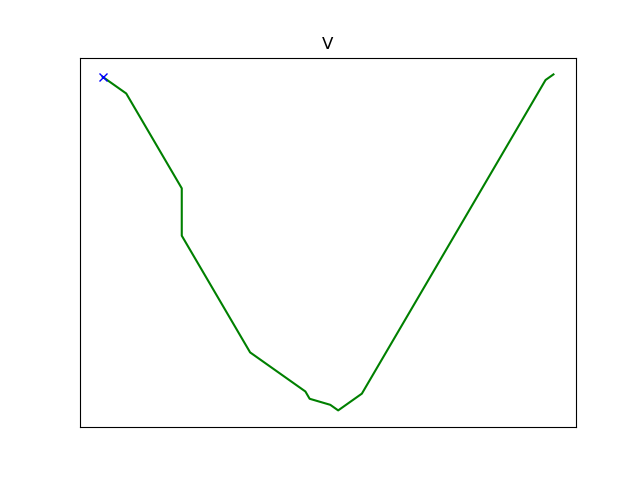
\includegraphics[width=\textwidth]{images/gbem/orig_letters_fig/AORIG_letter_V_writer_11.png}
        \caption{V}
    \end{subfigure}
    ~
    \begin{subfigure}[b]{0.14\textwidth}
        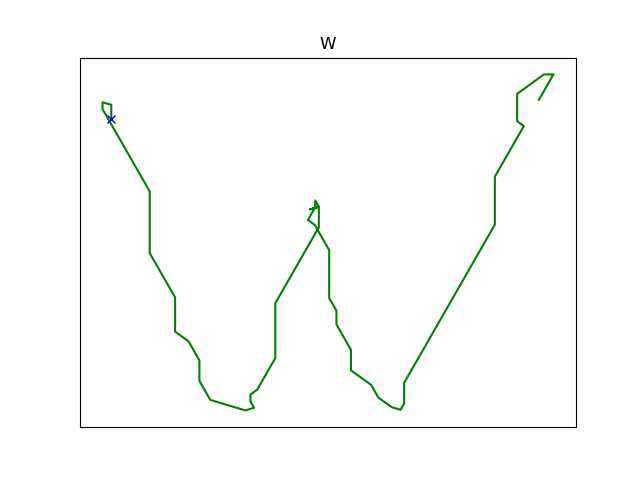
\includegraphics[width=\textwidth]{images/gbem/orig_letters_fig/AORIG_letter_W_writer_2.png}
        \caption{W}
    \end{subfigure}
    ~
    \begin{subfigure}[b]{0.14\textwidth}
        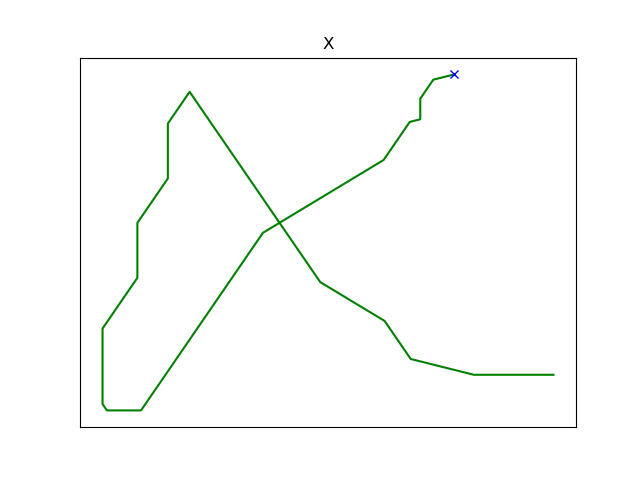
\includegraphics[width=\textwidth]{images/gbem/orig_letters_fig/AORIG_letter_X_writer_5.png}
        \caption{X}
    \end{subfigure}
    ~
    \begin{subfigure}[b]{0.14\textwidth}
        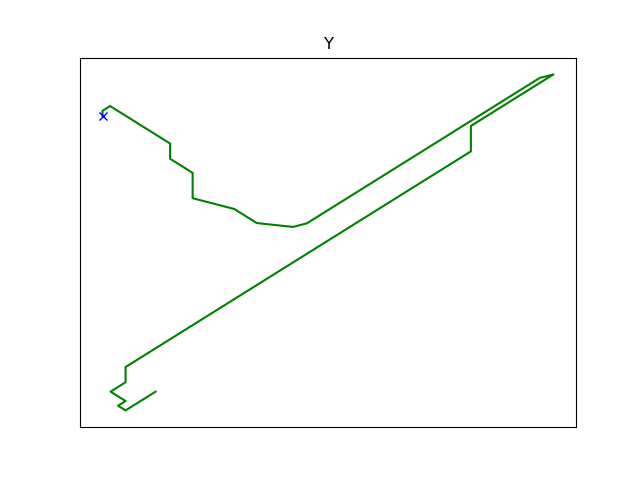
\includegraphics[width=\textwidth]{images/gbem/orig_letters_fig/AORIG_letter_Y_writer_5.png}
        \caption{Y}
    \end{subfigure}
    ~
    \begin{subfigure}[b]{0.14\textwidth}
        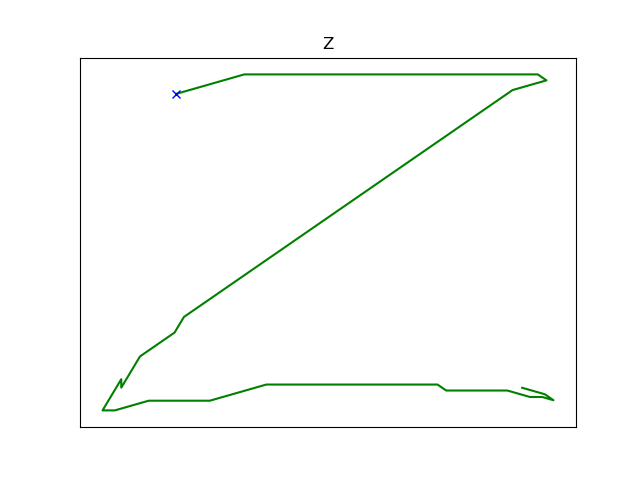
\includegraphics[width=\textwidth]{images/gbem/orig_letters_fig/AORIG_letter_Z_writer_15.png}
        \caption{Z}
    \end{subfigure}

    \caption{Examples of original letters. The blue \textit{x} mark is the starting point. These ones are generated using the letter + Writer bias. E and F are visually harder to recognize, since we do not model the pen pressure, otherwise, the rest of the letters are well recognizable.}\label{fig:orig_letters_examples}
\end{sidewaysfigure}

\begin{sidewaysfigure}[!htbp]
\centering
    \begin{subfigure}[b]{0.14\textwidth}
        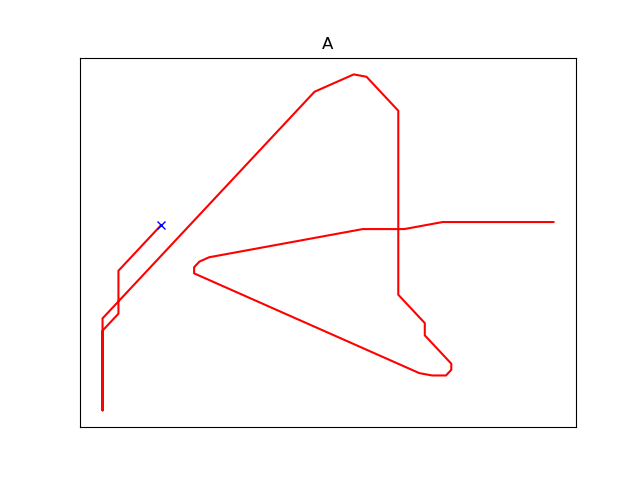
\includegraphics[width=\textwidth]{images/gbem/letters_generated/A.png}
        \caption{A}
    \end{subfigure}
    ~ %add desired spacing between images, e. g. ~, \quad, \qquad, \hfill etc.
      %(or a blank line to force the subfigure onto a new line)
    \begin{subfigure}[b]{0.14\textwidth}
        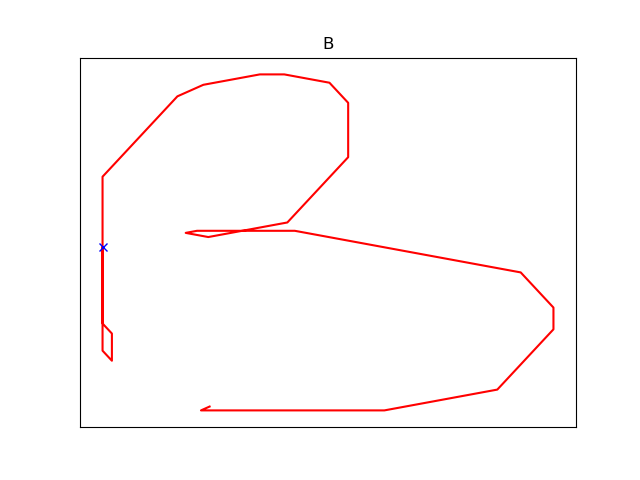
\includegraphics[width=\textwidth]{images/gbem/letters_generated/B.png}
        \caption{B}
    \end{subfigure}
    ~
    \begin{subfigure}[b]{0.14\textwidth}
        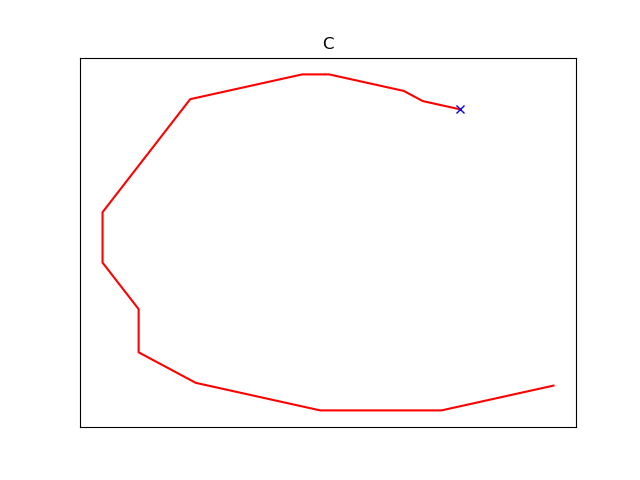
\includegraphics[width=\textwidth]{images/gbem/letters_generated/C.png}
        \caption{C}
    \end{subfigure}
    ~
    \begin{subfigure}[b]{0.14\textwidth}
        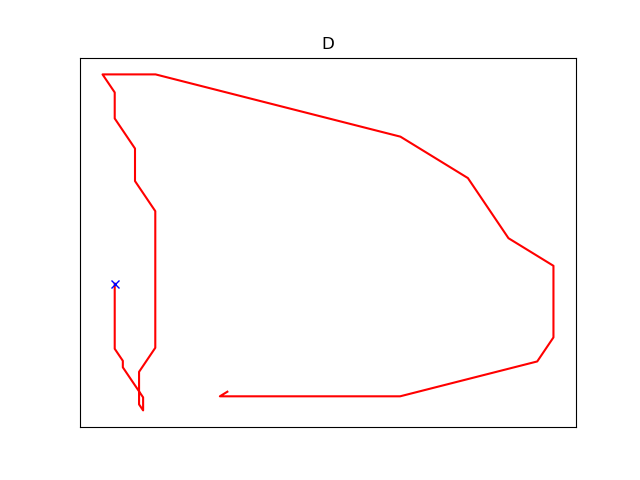
\includegraphics[width=\textwidth]{images/gbem/letters_generated/D.png}
        \caption{D}
    \end{subfigure}
    ~
    \begin{subfigure}[b]{0.14\textwidth}
        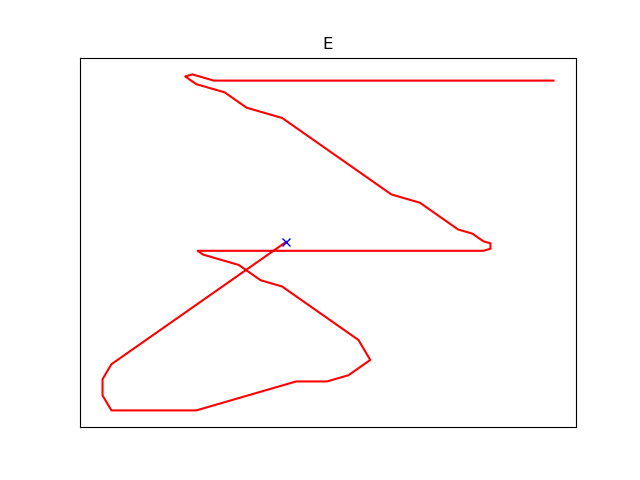
\includegraphics[width=\textwidth]{images/gbem/letters_generated/E.png}
        \caption{E}
    \end{subfigure}
    ~
    \begin{subfigure}[b]{0.14\textwidth}
        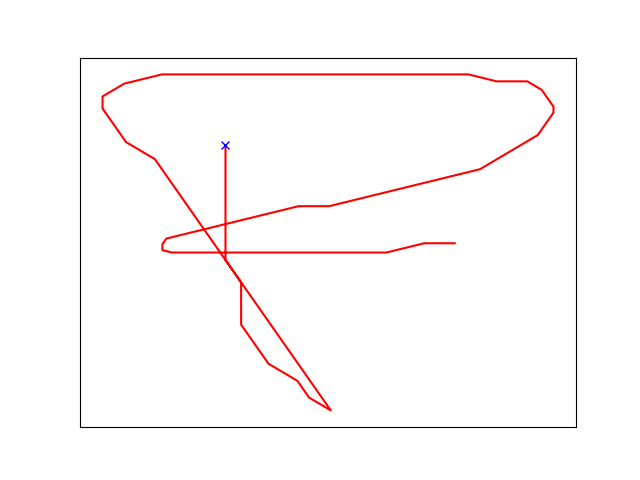
\includegraphics[width=\textwidth]{images/gbem/letters_generated/F.png}
        \caption{F}
    \end{subfigure}
    ~
    \begin{subfigure}[b]{0.14\textwidth}
        \includegraphics[width=\textwidth]{images/gbem/letters_generated/G.png}
        \caption{G}
    \end{subfigure}
    ~
    \begin{subfigure}[b]{0.14\textwidth}
        \includegraphics[width=\textwidth]{images/gbem/letters_generated/H.png}
        \caption{H}
    \end{subfigure}
    ~
    \begin{subfigure}[b]{0.14\textwidth}
        \includegraphics[width=\textwidth]{images/gbem/letters_generated/I.png}
        \caption{I}
    \end{subfigure}
    ~
    \begin{subfigure}[b]{0.14\textwidth}
        \includegraphics[width=\textwidth]{images/gbem/letters_generated/J.png}
        \caption{J}
    \end{subfigure}
    ~
    \begin{subfigure}[b]{0.14\textwidth}
        \includegraphics[width=\textwidth]{images/gbem/letters_generated/K.png}
        \caption{K}
    \end{subfigure}
    ~
    \begin{subfigure}[b]{0.14\textwidth}
        \includegraphics[width=\textwidth]{images/gbem/letters_generated/L.png}
        \caption{L}
    \end{subfigure}
    ~
    \begin{subfigure}[b]{0.14\textwidth}
        \includegraphics[width=\textwidth]{images/gbem/letters_generated/M.png}
        \caption{M}
    \end{subfigure}
    ~
    \begin{subfigure}[b]{0.14\textwidth}
        \includegraphics[width=\textwidth]{images/gbem/letters_generated/N.png}
        \caption{N}
    \end{subfigure}
    ~
    \begin{subfigure}[b]{0.14\textwidth}
        \includegraphics[width=\textwidth]{images/gbem/letters_generated/O.png}
        \caption{O}
    \end{subfigure}
    ~
    \begin{subfigure}[b]{0.14\textwidth}
        \includegraphics[width=\textwidth]{images/gbem/letters_generated/P.png}
        \caption{P}
    \end{subfigure}
    ~
    \begin{subfigure}[b]{0.14\textwidth}
        \includegraphics[width=\textwidth]{images/gbem/letters_generated/Q.png}
        \caption{Q}
    \end{subfigure}
    ~
    \begin{subfigure}[b]{0.14\textwidth}
        \includegraphics[width=\textwidth]{images/gbem/letters_generated/R.png}
        \caption{R}
    \end{subfigure}
    ~
    \begin{subfigure}[b]{0.14\textwidth}
        \includegraphics[width=\textwidth]{images/gbem/letters_generated/S.png}
        \caption{S}
    \end{subfigure}
    ~
    \begin{subfigure}[b]{0.14\textwidth}
        \includegraphics[width=\textwidth]{images/gbem/letters_generated/T.png}
        \caption{T}
    \end{subfigure}
    ~
    \begin{subfigure}[b]{0.14\textwidth}
        \includegraphics[width=\textwidth]{images/gbem/letters_generated/U.png}
        \caption{U}
    \end{subfigure}
    ~
    \begin{subfigure}[b]{0.14\textwidth}
        \includegraphics[width=\textwidth]{images/gbem/letters_generated/V.png}
        \caption{V}
    \end{subfigure}
    ~
    \begin{subfigure}[b]{0.14\textwidth}
        \includegraphics[width=\textwidth]{images/gbem/letters_generated/W.png}
        \caption{W}
    \end{subfigure}
    ~
    \begin{subfigure}[b]{0.14\textwidth}
        \includegraphics[width=\textwidth]{images/gbem/letters_generated/X.png}
        \caption{X}
    \end{subfigure}
    ~
    \begin{subfigure}[b]{0.14\textwidth}
        \includegraphics[width=\textwidth]{images/gbem/letters_generated/Y.png}
        \caption{Y}
    \end{subfigure}
    ~
    \begin{subfigure}[b]{0.14\textwidth}
        \includegraphics[width=\textwidth]{images/gbem/letters_generated/Z.png}
        \caption{Z}
    \end{subfigure}

    \caption{Examples of generated letters. The blue \textit{x} mark is the starting point. These ones are generated using the letter + Writer bias. The general quality of this quite acceptable.}
    \label{fig:letters_examples_gbem}
\end{sidewaysfigure}


\section{Summary}

\par In this chapter, we sit the foundations for the work done in our thesis. We first discussed the relevant areas in the state-of-the-art concerning recurrent neural networks, optimization, inference/generation and evaluation of generation. We then detailed how we combine these elements in order to address the questions in this thesis. We addressed three points:
\begin{itemize}
    \item How to generate traces using deep generative models? We proposed to use a conditioned-GRU model. We explained the process behind training, optimizing and choosing hyper-parameters for this model, and showed some of the generated letters.
    \item How to evaluate the quality of the generated letters? We proposed two evaluation criteria, BLEU score metric -- inspired by its usage in evaluating text quality -- and End-of-Sequence quality, as a way to capture some aspects of the distribution, and a feasible way to measure the distance between two distributions.
    \item We proposed multiple benchmarks for future evaluation of style extraction models, and to ground the proposed evaluation metrics as well.
\end{itemize}
Now that we have our benchmarks and evaluation metrics, it is time to go for the next chapter on style extraction.
